% -------- VARIABLES -------------------------------------------------------
\newcommand{\lectureVar}{Rechnersysteme \& -Netze}
\newcommand{\moduleVar}{Systeme 1}
\newcommand{\semesterVar}{WiSe 20/21}
\newcommand{\authorVar}{Noah Kamara}



% -------- PACKAGES --------------------------------------------------------
% Document Class
\documentclass[12pt]{report}

% Page Layout & Formatting
\usepackage[a4paper,width=150mm,top=25mm,bottom=25mm,left=20mm,right=20mm]{geometry} % Layout
\usepackage{fancyhdr} % Headers
\usepackage{titlesec} % Titles
\usepackage[many]{tcolorbox} % Boxes (Definitions, Examples)
\usepackage{graphicx} % Images / Other Graphics
\graphicspath{{../graphics/}}
\usepackage{float} % Floats (like Minipage) alignment
\usepackage{parskip} % no indents in new par
\usepackage[hidelinks]{hyperref} % Hyperrefs
\usepackage{bookmark}% Bookmarks

% Math Mode
\usepackage{amsmath}
\usepackage{cancel}

% Language Specific
\usepackage[utf8]{inputenc}
\usepackage[german]{babel} 

% Tables & Arrays
\usepackage{array}   % column types / tables
\usepackage{multicol} % tables, multicolumn

\usepackage{caption} % Caption styling
\usepackage{xcolor}



% -------- HEADERS, FOOTERS & TITLES ---------------------------------------
\pagestyle{fancy}
\fancyhf{}

\renewcommand{\chaptermark}[1]{\markboth{#1}{}}
\renewcommand{\headrulewidth}{1pt}
\renewcommand{\footrulewidth}{1pt}

% Header
\setlength{\headheight}{30pt}
\lhead{\moduleVar\\\lectureVar}
\rhead{\semesterVar\\\authorVar}

% Footer
\cfoot{\thepage}

% Titles
\titleformat{\section}[display]{\normalfont\bfseries}{}{0pt}{\Huge}



% -------- MATH MODE -------------------------------------------------------
% Math Mode Table Columns
\newcolumntype{L}{>{$}l<{$}}
\newcolumntype{C}{>{$}c<{$}}

% Überträge
\def\cred{\hbox to0pt{\textcolor{blue}{${}_{\tt 1}$}\hss}}



% -------- COLORS ----------------------------------------------------------
% Text Colors
\definecolor{mainColor}{HTML}{121113}
\definecolor{secColor}{HTML}{222725}

% ColorBox Colors
\definecolor{defboxColor}{HTML}{B5D99C}
\definecolor{infoboxColor}{HTML}{FFFF82}
\definecolor{boxbgColor}{HTML}{F2F2F2}
\definecolor{warnboxColor}{HTML}{FF0000}


% -------- Color Boxes ----------------------------------------------------- 
% Definition Box
\newtcolorbox{defbox}[1][]{
	title=\textbf{DEFINITION:  #1},
  boxrule = 1.5pt,
  rounded corners,
	arc = 5pt,
  coltitle = mainColor,
  colframe = defboxColor,
  colback = boxbgColor
}

% Info Box
\newtcolorbox{infobox}[1][]{
	title=\textbf{INFO: #1},
  boxrule = 1.5pt,
  rounded corners,
	arc = 5pt,
	coltitle = mainColor,
	colframe = infoboxColor,
  colback = boxbgColor
}

% Example Box
\newtcolorbox{exbox}[1][]{
	title=\textbf{BEISPIEL: #1},
  boxrule = 1.5pt,
  rounded corners,
	arc = 5pt,
  colback = boxbgColor
}

% Warninng Box
\newtcolorbox{warnbox}[1][]{
	title=\textbf{BEISPIEL: #1},
  boxrule = 1.5pt,
  rounded corners,
	arc = 5pt,
  coltitle = mainColor,
	colframe = warnboxColor,
  colback = boxbgColor
}




\begin{document}

\tableofcontents

\chapter{Schaltungstechnik I}

\section{Boolesche Algebra / Schaltalgebra}

\begin{defbox}[Boolesche Algebra]
  Eine \textit{Boolesche Algebra} ist eine Menge B mit dem Nullelement 0 und dem
  Einselement 1 (d.h., $0, 1 \in B$), auf der die Operationen \textbf{Konjunktion} $\wedge$ und  \textbf{Disjunktion} $\vee$ sowie \textbf{Negation} $\neg$ definiert sind.
\end{defbox}

\begin{defbox}[Schaltalgebra]
  Eine \textit{Schaltalgebra} ist eine Boolesche Algebra mit der Trägermenge $B=\{0,1\}$.
\end{defbox}

\subsection{Axiomensystem}

\begin{table}[H]
  \begin{tabular}{ccc}
    \multicolumn{3}{c}{\textbf{George Boole (1847)}}                                                                               \\
    Kommutativität   & $a \wedge b = b \wedge a$                             & $a \vee b = b \vee a$                               \\
    Assoziativität   & $(a \wedge b) \wedge c = a \wedge (b \wedge c)$       & $(a \vee b) \vee c = a \vee (b \vee c)$             \\
    Idempotenz       & $ a \wedge a = a$                                     & $ a \vee a = a$                                     \\
    Distributivität  & $a \wedge (b\vee c) = (a \wedge b) \vee (a \wedge c)$ & $a \vee (b\wedge c) = (a \vee b) \wedge (a \vee c)$ \\
    Neutralität      & $a \wedge 1 = a$                                      & $a \vee 0 = a$                                      \\
    Extremalität     & $a \wedge 0 = 0$                                      & $a \vee 1 = 1$                                      \\
    Involution       & $\neg \neg a = a$                                     &                                                     \\
    \multicolumn{3}{c}{\textbf{De Morgan (1860)}}                                                                                  \\ 
    De Morgan        & $\neg(a \wedge b) = \neg a \vee \neg b$               & $\neg(a \vee b) = \neg a \wedge \neg b$             \\
    Komplementarität & $ a \wedge \neg a = 0$                                & $a \vee \neg a = 1$                                 \\
    Dualität         & $\neg 0 = 1$                                          & $\neg 1 = 0$                                        \\
    Absorption       & $a \vee (a \wedge b) = a$                             & $a \wedge ( a \vee b) = a$
  \end{tabular}
\end{table}


\subsection{Boolesche Funktionen}
\begin{defbox}[Boolesche Funktionen]
  Eine Boolesche Funktion ist eine Funktion $f : \{0, 1\}n \rightarrow \{0, 1\}, n \geq 0$.
  Die Anzahl $n$ der Argumente der Funktion $f$ heißt ihre Stelligkeit (arity).

  Für kleine Stelligkeiten gibt es Spezielle Ausdrücke:
  \begin{itemize}
    \item $n=1$: \textbf{unär} (unary)
    \item $n=2$: \textbf{binär} (binary)
    \item $n=3$: \textbf{ternär} (ternary)
  \end{itemize}

  Boolesche Funktionen werden durch \textbf{Schaltnetze} implementiert.
\end{defbox}

Jede Boolesche Funktion kann durch \textbf{Wahrheitstafeln} und \textbf{Formeln der Schaltalgebra} dargestellt werden.

\subsubsection{Darstellung durch Wahrheitstafeln}
\begin{figure}[H]
  \begin{minipage}[t]{0.5\textwidth}
    \begin{itemize}
      \item eine Spalte pro Funktionsargument,
      \item eine Zeile pro mögliche Wertekombination der Funktionsargumente,
      \item zusätzliche Spalte für den Funktionswert.
    \end{itemize}
  \end{minipage}
  \hfill
  \begin{minipage}[t]{0.4\textwidth}
    \caption{Wahrheitstafel einer ternären Booleschen Funktion}
    \centering
    \begin{tabular}{ccc|c}
      $x_1$ & $x_2$ & $x_3$ & $y$  \\ \hline
      0     & 0     & 0     & 0    \\
      1     & 0     & 0     & 1    \\
      0     & 1     & 0     & 1    \\
      0     & 0     & 1     & 0    \\
      1     & 0     & 1     & 1    \\
      0     & 1     & 1     & 0    \\
      1     & 1     & 1     & 1   
    \end{tabular}
  \end{minipage}
\end{figure}

\subsubsection{Darstellung durch Formeln der Schaltalgebra}
\begin{figure}[H]
  \begin{minipage}{0.46\textwidth}
    \paragraph{Disjunktive Normalform}
    \begin{itemize}
      \item[$\rightarrow$] Darstellung der Minterme
      \item[$\rightarrow$] Sum of Products (SOP)
    \end{itemize}
    Bilde \textit{Disjunktion der Konjunktionen} aus Literalen aus jeder Zeile in der der Funktionswert 0 ist
  \end{minipage}
  \hfill
  \begin{minipage}{0.46\textwidth}
    \paragraph{Konjunktive Normalform}
    \begin{itemize}
      \item[$\rightarrow$] Darstellung der Maxterme
      \item[$\rightarrow$] Product of Sums (POS)
    \end{itemize}
    Bilde \textit{Konjunktion der Disjunktionen} aus Literalen aus jeder Zeile in der der Funktionswert 1 ist
  \end{minipage}
\end{figure}

\paragraph{Konjunktive und Disjunktive Normalform im Vergleich:}
Bevorzuge die disjunktive bei weniger Einsen, die konjunktive
bei weniger Nullen in den Funktionswerten.
% TODO: Add Example

\subsubsection{Vollständige Operationenmengen}
\begin{defbox}[Vollständige Operationenmengen]
  Eine vollständige Operationenmenge ist eine Menge von Booleschen Operationen, die ausreicht, um alle Booleschen Funktionen darzustellen
\end{defbox}
Da sowohl die disjunktive als auch die konjunktive Normalform nur die Operationen Konjunktion, Disjunktion und Negation benutzt, ist die Menge $O=\{ \vee, \wedge, \neg\}$ eine vollständige Operationenmenge.
\par Von einer anderen Operation $O'$ kann man zeigen, dass sie vollständig ist, indem man die drei Operationen von $O$ nur mit Hilfe der Operationen aus dieser Menge $O'$ darstellt.


\section{Gatterlogik}
\begin{defbox}[(Logik-)Gatter]
  Ein Logikgatter ist eine Anordnung zur Realisierung einer booleschen Funktion, die binäre Eingangssignale zu einem binären Ausgangssignal verarbeitet.
  Die Eingangssignale weerden durch Implementierung logischer Operatoren zu einem einzigen logischen Ergebnis umgewandelt.
\end{defbox}

\subsection{Implementierung}
Boolesche Funktionen werden mit Hilfe der Gatterlogik implementiert. 
Das heißt, mehrere elementare Gatter werden zusammengeschaltet, um komplexe Boolesche Funktionen zu berechnen:
% TODO Elementare Gatter & Zusammengesetze Gatter

\subsubsection{Vollständige Operationenmengen}
% TODO NAND, zeige Vollständigkeit

\subsubsection{Datenflußsteuerung}
Wir können den Fluss von Daten mit sogenannten Steuerleitungen kontrollieren:
Wir nehmen an:
\begin{itemize}
  \item Datensignal $d$ läuft auf einer \textit{Datenleitung} $D$
  \item Steuersignal $c$ läuft auf einer \textit{Steuerleitung} $C$
\end{itemize}

Nur wenn auf Steuerleitung $C$ eine logische 1 anliegt, soll das Datensignal weitergeleitet werden.
Das ist mit einem AND-Gatter einfach zu implementieren: 
% REPLACE FROM HERE
Wir benutzen ein AND-Gatter und verbinden D und C zu einem gemeinsamen Ausgangssignal, 
an dem dann eine logische 1 anliegt, wenn an Datenleitung D eine 1 anliegt und Steuerleitung C 
ebenfalls auf 1 steht
% TODO REPLACE DRAWING 

\subsection{Multiplexer (Auswahlschaltung)}
01 - 31ff

\subsection{2-Bit-Dekodierer}



\section{Implementierung von Schaltnetzen}
\begin{defbox}
  Durch elektronische Bauteile, speziell (Feldeffekt-)Transistoren, werden spannungsgesteuerte Schalter dargestellt.
  aus mehreren Schaltern werden dann Gatter zusammengesetzt, die einfache Boolesche Funktionen darstellen.
  Die Gatter bilden jeweils eine vollständige Operationenmenge.
\end{defbox}

\subsection{Elektronische Grundlagen}
\subsubsection{Schalter}
Um Gatter zu implementieren werden Schalter benötigt, die automatisch betätigt werden können. Hierzu gibt es nun mehrere Ansätze:
\begin{itemize}
  \item Erste Lösung: \textit{Relais}: (elektromechanische/magnetische
        Schalter)\\
        Relativ groß, hoher Stromverbrauch, Mechanisch und deshalb Störungsanfällig

  \item Bessere Lösung: \textit{Vakuumröhren}: (Verstärkerröhren) \\
        Immernoch groß aber geringerer Stromverbrauch

  \item Entscheidente Verbesserung: \textit{Transistoren}: (Halbleiterschalter/verstärker) \\
        Sehr klein \& kleiner Stromverbrauch

\end{itemize}


\subsubsection{Transistoren}
\begin{figure}[H]
  \begin{minipage}{0.45\textwidth}
    \textbf{Bipolartransistor}
    \par (bipolar junction transistor)
    \begin{itemize}
      \item[$\rightarrow$] 3 Anschlüsse:
            \begin{itemize}
              \item Basis (base)
              \item Emitter (emitter)
              \item lektor (collector)
            \end{itemize}
      \item[$\rightarrow$] stromgesteuert

            Kleiner Steuerstrom auf der Basis-Emitter-Strecke steuert großen Strom auf Kollektor-Emitter-Strecke.
    \end{itemize}
  \end{minipage}
  \hfill
  \begin{minipage}{0.45\textwidth}
    \textbf{Feldeffekttransistor}
    \par (field effect transistor)
    \begin{itemize}
      \item[$\rightarrow$] 3 Anschlüsse:
            \begin{itemize}
              \item Quelle (source)
              \item Senke (drain)
              \item Steuerelektrode (gate)
            \end{itemize}
      \item[$\rightarrow$] spannungsgesteuert

            Der Widerstand und somit der Strom der Drain-Source-Strecke wird durch die Gate-Source-Spannung gesteuert. Im statischen Fall fasst Stromlos
    \end{itemize}
  \end{minipage}
\end{figure}

$\rightarrow$ Wir beschränken uns im Folgenden auf Feldeffekttransistoren, da diese für Rechnertechnik (und speziell für integrierte Schaltunngen) wesentlich wichtiger sind


\subsubsection{Feldeffekttransistoren}
%TODO: CONTINUE WITH 01 - Schaltungstechnik I p34

\subsubsection{Transistorschalter}




\chapter{Schaltungstechnik II}
\section{Minimierung Boolescher Formeln}
\begin{defbox}[Semantische \& Syntaktische Äquivalenz]
  Seien $\varphi$ und $psi$ Boolesche Formeln, dann gilt:

  \begin{itemize}
    \item Wenn beide Formeln für alle Belegungen den gleichen Wahrheitswert haben, dann sind die Formeln

          \center{\textit{Semantische äquivalent}: $\varphi \equiv \psi$}


    \item Wenn $\varphi$ durch Äquivalenzumformungen in $\psi$ umgeformt werden kann, dann sind die Formeln

          \center{\textit{Syntaktische äquivalent}: $\varphi = \psi$}
  \end{itemize}
\end{defbox}

Für die Syntaktische Äquivalenz ist der Nachweis oft wesentlich kürzer. Ein Abschluss der Äquivalenzprüfung ist allerdings nicht garantiert (kein Weg gefunden $\not \rightarrow$ $\varphi \not \equiv \psi$).
Für die Semantische Äquivalenz kann der Nachweis sehr aufwendig sein. Zum Falsifizieren wird jedoch lediglich eine Wertkombination benötigt, die nicht equivalent ist.

\subsection{Äquivalenzumformungen}
Die Axiome der Booleschen Algebra erlauben es, alle semantische geltenden Äquivalenten auf syntaktischem Wege abzuleiten, denn es gilt:

\begin{center}
  Zwei Boolesche Formeln sind \textbf{genau dann} semantisch äquivalent, wenn sie syntaktisch äquivalent sind.
\end{center}


\subsection{Systematische Vereinfachungsverfahren}
Das Problem Äquivalenzumformungen ist, dass es keine klare Strategie zur Vereinfachung gibt.
Besser wäre ein systematisches Vereinfachungsverfahren.

\subsubsection{Karnaugh-Veitch-Diagramme}
\begin{defbox}[Karnaugh-Veitch-Diagramme]
  Tabellarische Darstellungen Boolescher
  Funktion (wie Wahrheitstafeln, nur andere Auflistung der Funktionswerte).
  \begin{itemize}
    \item $2^n$ Felder für $n$ Argumente.
    \item Anordung, dass ein Übergang zu einem Nachbarfeld den Wert nur genau einer der Variablen ändert (ein sog. Gray-Code)
  \end{itemize}
\end{defbox}

\begin{exbox}[Zwei Variablen]
  \begin{minipage}{0.6\textwidth}
    Ein Gray-Code für zwei Variablen:

    Anordnung ist bis auf zyklische Vertauschungen und Spiegelungen eindeutig.
  \end{minipage}
  \hfill
  \begin{minipage}{0.3\textwidth}
    \begin{tabular}{cccc}
      00 & 01 & 11 & 10 \\
      01 & 11 & 10 & 00 \\
      11 & 10 & 00 & 01 \\
      10 & 00 & 11 & 10 \\
    \end{tabular}
  \end{minipage}
\end{exbox}
Sind zwei benachbarte Felder eines Karnaugh-Veitch-Diagramms beide 1, so zeigt dies an, dass eine bestimmte Variable in der ursprünglichen Funktion irrelevant ist.
Beim Zusammenfassen von Feldern darf auch der Rand überschritten werden, da sich auch in diesem Fall der Wert nur einer Variable ändert:
Wie oben gezeigt können auch mehr als 2 Felder Zusammengefasst werden, jedoch nur, wenn die Felderzahlen Zweierpotenzen sind.

\begin{figure}[h]
  \caption{Beispiel für Karnaugh-Veitch-Diagramms}
  \centering
  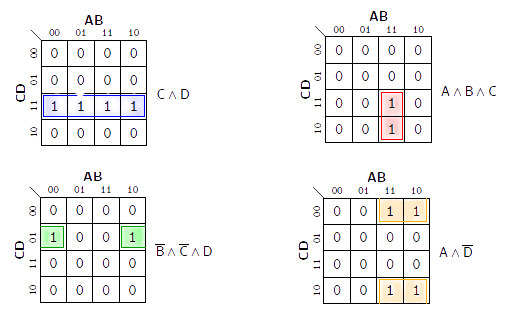
\includegraphics[width=\textwidth]{karnaugh-veitch-example01}
\end{figure}


\begin{enumerate}
  \item \textbf{Schritt:}
        Finde alle maximalen Zusammenfassungen von Feldern

        (dürfen überlappen, aber nicht in größeren Zusammenfassungen vorkommen)

        \begin{center}
          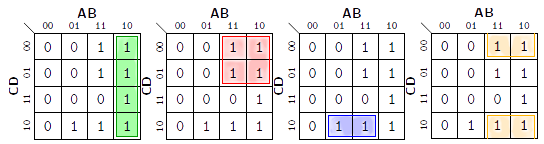
\includegraphics[scale=1]{karnaugh-veitch-step_01}
        \end{center}


  \item \textbf{Schritt:}
        Wähle möglichst wenige Zusammenfassungen, die alle Einsen abdecken

        \begin{center}
          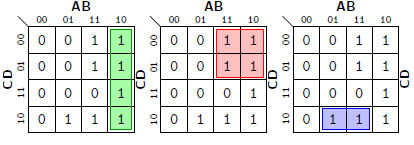
\includegraphics[scale=1]{karnaugh-veitch-step_02}
        \end{center}


  \item \textbf{Schritt:}
        Sammle die benötigten Ausdrücke:
        \begin{multicols}{2}
          \begin{align*}
            0 & = \color{red}{(A \wedge \overline{C})}              \\
              & \vee \color{green}{(A \wedge B)}                    \\
              & \vee \color{blue}{(B \wedge C \wedge \overline{D})}
          \end{align*}
          \columnbreak
          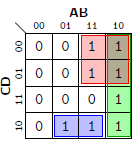
\includegraphics[scale=1]{karnaugh-veitch-step_03}
        \end{multicols}
\end{enumerate}

\begin{infobox}
  Natürlich kann die Minimierung nicht nur durch Zusammenfassen von Einsen, sondern, 
  unter Rückgriff auf die Dualität der Booleschen Gesetze bzw. 
  die Dualität der disjunktiven und der konjunktiven Normalform, 
  auch durch Zusammenfassen von Nullen durchgeführt werden.

  Da das Ergebnis eine Konjunktion von Disjunktionen ist (analog zur konj. Normalform) 
  müssen die Variablenwerte, 
  die die Zusammenfassungen beschreiben negiert werden
\end{infobox}
\subsubsection{Quine-McCuskey-Algorithmus}
Eine Minimierung logischer Funktionen mit bis zu sechs Argumenten ist zwar mit erweiterten 
Karnaugh-Veitch-Diagrammen im Prinzip möglich, aber unhandlich. Ein besserer Weg besteht 
in der Verwendung eines anderen Verfahrens des \textbf{Quine-McClunskey-Algorithmus}.

\begin{enumerate}
  \item \textbf{Schritt:} Bilde die disjunktive (analog auch konmjunktive) Normalform der zu minimierenden Funktion.
  \item \textbf{Schritt:} Finden der \textbf{Primimplikanten} (Abb. \ref{fig:Quine–McCluskeyAlgorithmus_step_01}).
        \begin{itemize}
          \item Vereinige Terme, in denen eine einzelne Variable
                in dem einen Term als positives, im anderen als negatives Literal auftritt.
                (Der gleiche Term darf für mehrere Vereinigungen verwendet werden.)

                \begin{align*}
                  (A_1 ... A_i ... A_n) \vee (A_1 ... \overline{A_i} ... A_n)
                   & = A_1 ... A_{i-1} A_{i+1} ... A_n \wedge (A_i \vee \overline{A_i})  \\
                   & = A_1 ... A_{i-1} A_{i+1} ... A_n \wedge 1                          \\
                   & = A_1 ... A_{i-1} A_{i+1} ... A_n                                  
                \end{align*}
          \item Wiederhole dies Rekursiv mit den Vereinigungsergebnissen, bis keine weiteren Vereinigungen mehr möglich sind.
          \item Vernachlässige alle Terme, die mit anderen Vereinigt wurden.
          \item Übrig bleiben die sogenannten \textbf{Primimplikanten}
        \end{itemize}

        \begin{figure}[H]
          \caption{Tabelle zur bestimung von Primimplikanten}
          \label{fig:Quine–McCluskeyAlgorithmus_step_01}
          \centering
          \includegraphics[width=\textwidth]{Quine–McCluskeyAlgorithmus_step_01}
        \end{figure}

  \item \textbf{Schritt:} Aufstellen und Auswerten der Primimplikantentabelle
        \begin{itemize}
          \item Spalten: Minterme, Zeilen: Primimplikanten
          \item Finde wesentliche Primimplikanten (aufsuchen der Spalten mit nur einer Markierung)

                Eine systematische Methode für diese Auswahl von Primimplikanten ist \textbf{Petricks Algorithmus}
        \end{itemize}
        \begin{center}
          \includegraphics[scale=1]{Quine–McCluskeyAlgorithmus_step_02}
        \end{center}

        \begin{itemize}
          \item[\color{red} $\bullet$ ] Abdeckung nur durch einen Primimplikanten $\rightarrow$ wesentlich
          \item[\color{blue} $\bullet$ ] Abdeckung auch durch wesentliche Primimplikanten.
          \item[\color{gray} $\bullet$ ] Nicht benötigte Abdeckungen
        \end{itemize}
\end{enumerate}


\begin{infobox}
  Primimplikanten des Quine-McCluskey-Algorithmus entsprechen 
  Feld-Zusammenfassungen in Karnaugh-Veitch-Diagrammen.

  Dementsprechend gibt es auch wesentliche Zusammenfassungen in Karnaugh-Veitch-Diagrammen. 
  (Feldergruppen, die von keiner der anderen Gruppen abgedeckt werden)
\end{infobox}
\begin{figure}[h]
  \begin{minipage}{0.6\textwidth}
    \begin{itemize}
      \item[\color{green} Grün] entspricht dem 4er Primimplikanten 10--
      \item[\color{red} Rot\ ] entspricht dem 4er Primimplikanten -110
      \item[\color{blue} Blau] entspricht dem 2er Primimplikanten -110
      \item[\color{yellow} Gelb] entspricht dem 4er Primimplikanten 1--0
    \end{itemize}
  \end{minipage}
  \hfill
  \begin{minipage}{0.4\textwidth}
    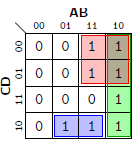
\includegraphics{karnaugh-veitch-step_03}
  \end{minipage}
\end{figure}

\subsection{Petricks Algorithmus}
Nicht immer decken die wesentlichen Primimplikanten alle Minterme ab. 
In diesem Fall müssen aus den restlichen Primimplikanten geeignete ausgewählt werden, 
um die verbleibenden Minterme abzudecken.


\begin{enumerate}
  \item \textbf{Schritt:} Bilde eine reduzierte Primimplikantentabelle

        Diese enthält nur noch die noch nicht abgedeckten Minterme und die nicht wesentlichen Primimplikanten.

  \item \textbf{Schritt:} Ordne jedem Primimplikanten eine Auswahlvariable $P_i$ zu.

  \item \textbf{Schritt:} Bilde für jeden Minterm (Spalte) die Disjunktion der Auswahlvariablen.

        Alle Primimplikanten, die diesen Minterm abdecken werden mit einer Disjunktion verknüpft.

  \item \textbf{Schritt:} Verknüpfe alle Disjunktionen zu einer Konjunktion $C$.

  \item \textbf{Schritt:} Wandle Konjunktion $C$ durch die Distributivgesetze in eine Disjunktion $D'$ um

        Nun ergibt sich eine Disjunktion aus Konjunktionen, die jeweils alle Minterme abdecken.
        $$(P_1 \wedge P_2 \wedge P_3) \vee (P_2 \wedge P_3 \wedge P_4) \vee (P_3 \wedge P_5)$$

  \item \textbf{Schritt:} Wähle die Konjunktionen aus $D'$, mit den wenigsten Primimplikanten

        $P_3 \wedge P_5$

\end{enumerate}

\begin{figure}[H]
  \begin{minipage}{0.6\textwidth}
    \begin{table}[H]
      \centering
      \begin{tabular}{|cc|cccccl|}
        \hline
                                              &     & \multicolumn{6}{c|}{Minterme (Konjunktionen)}                                                                                                                              \\ \hline
        \multicolumn{2}{|c|}{Primimplikanten} & 000 & 001                                           & 010                    & 101                    & 110                    & 111                                             \\ \hline
        \multicolumn{1}{|c|}{$P_1$}           & 00- & \color{blue} $\bullet$                        & \color{blue} $\bullet$ &                        &                        &                        &                        \\
        \multicolumn{1}{|c|}{$P_2$}           & 0-0 & \color{blue} $\bullet$                        &                        & \color{blue} $\bullet$ &                        &                        &                        \\
        \multicolumn{1}{|c|}{$P_3$}           & -01 &                                               & \color{blue} $\bullet$ &                        & \color{blue} $\bullet$ &                        &                        \\
        \multicolumn{1}{|c|}{$P_4$}           & -10 &                                               &                        & \color{blue} $\bullet$ &                        & \color{blue} $\bullet$ &                        \\
        \multicolumn{1}{|c|}{$P_5$}           & 1-1 &                                               &                        &                        & \color{blue} $\bullet$ &                        & \color{blue} $\bullet$ \\
        \multicolumn{1}{|c|}{$P_6$}           & 11- &                                               &                        &                        &                        & \color{blue} $\bullet$ & \color{blue} $\bullet$ \\ \hline
      \end{tabular}
    \end{table}
  \end{minipage}
  \begin{minipage}{0.4\textwidth}
    \begin{align*}
             & (P_1 \vee P_2)\ (001)   \\
      \wedge & (P_1 \vee P_3)\ (001) & \\
      \wedge & (P_2 \vee P_4)\ (010) & \\
      \wedge & (P_3 \vee P_5)\ (101) & \\
      \wedge & (P_4 \vee P_6)\ (110) & \\
      \wedge & (P_5 \vee P_6)\ (111) & \\
    \end{align*}
  \end{minipage}
\end{figure}


\section{Programmierbare Logikarrays}
Alle betrachteten Minimierungsergebnisse haben die folgende allgemeine Form:
$$o = (i_1 \wedge \overline{i_2} \wedge \overline{i_3} \wedge ...) \vee (\overline{i_1} \wedge i_2 \wedge \overline{i_3} \wedge ...) \vee (\overline{i_1} \wedge \overline{i_2} \wedge i_3 \wedge ...) \vee ... $$
Alle Boolesche Formeln können in diese Form gebracht werden, denn es handelt sich um eine Disjunktion von Konjunktionen von Literalen (sum of products, SOP)

\begin{defbox} [Programmierbare Logikarrays]
  Programmierbare Logikarrays (programmable logic array, PLAs) sind solche Formeln "realisiert in Hardware".
  \begin{itemize}
    \item Alle Eingaben $i_k$ und ihre Negation $\overline{i_k}$ sind verfügbar
    \item Die Eingaben werden über AND-Gatter verknüpft
    \item Die Ausgaben der AND-Gatter werden durch OR-Gatter verknüpft
    \item Ein PLA wird durch Entfernen von Verbindungen "konfiguriert" ("programmiert")
  \end{itemize}
\end{defbox}

\subsubsection{Gatterimplementierung von Originalfunktion und disjunkt. Normalform}

\begin{figure}[H]
  \begin{minipage}[t]{0.4\textwidth}
    \caption{Mehr Gatter, aber standardisierte Struktur}
    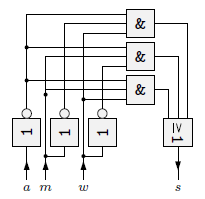
\includegraphics[width=\textwidth]{PLA_example_normal}
  \end{minipage}
  \hfill
  \begin{minipage}[t]{0.4\textwidth}
    \caption{Weniger Gatter, Struktur abhängig von Funktion}
    \centering
    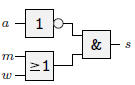
\includegraphics[width=\textwidth]{PLA_example_original}
  \end{minipage}
\end{figure}



\subsection{Allgemeine Struktur}
Jede Funktion in disjunktiver Normalform kann durch eine Standard-Gatterstruktur dargestellt werden:
\begin{itemize}
  \item Einem NOT-Gatter (Inverter), sodass für jede Eingabe negiert und unnegiert zur verfügung steht.
  \item Einem AND-Array, zur Berechnung der Konjunktionen
  \item Einem OR-Array, zur disjunktiven Verknüpfung der Konjunktionen
\end{itemize}


\subsection{Hardware-Implementation}

\begin{figure}[h]
  \begin{minipage}[t]{0.45\textwidth}
    \caption{Originale Darstellung von Schaltungen}
    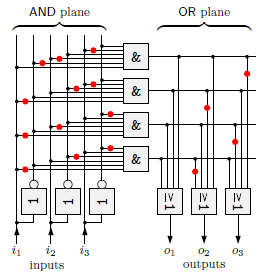
\includegraphics[height=\textwidth]{PLA_implementation}
    Bei Auslieferung sind Logikarrays komplett verbunden (an jedem UND-Gatter liegen alle negierte und unnegierte Eingaben an).
    Beim "programmieren" des Logikarrays werden die rot markierten Verbindungen getrennt
  \end{minipage}
  \hfill
  \begin{minipage}[t]{0.45\textwidth}
    \caption{Vereinfachte Darstellung von Schaltungen}
    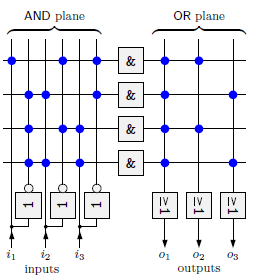
\includegraphics[height=\textwidth]{PLA_implementation_simplification}
    Zur Vereinfachung stellt man nur eine Linie je Gatter dar und markiert die \textbf{Verbindungen}
  \end{minipage}
\end{figure}

Für eine elektronische Implementierung (durch Transistoren) sind AND- und OR-Gatter nicht besonders gut geeignet.
Besser geeignet sind NAND- und NOR-Gatter (und ggf. NOT-Gatter).


\section{Hardware-Beschreibungssprache}
\begin{defbox}[Hardware-Beschreibungssprache]
  Eine formale Sprache, mit der Operationen von integrierten Schaltungen und ihr Design beschrieben sowie in Simulationen getestet werden können.
  \begin{itemize}
    \item Spezifieren von dem Verhalten von Bausteinen (Schnittstelle), sowie Implementierung aus Elementargattern.
    \item Simulator kann Elementargatter (und damit inderekt alle aus diesen zusammengesetzten Bausteine) simulieren
    \item Simuliertes Verhalten kann automatisch mit Schnittstelle verglichen werden (\textit{automatische Fehlerüberprüfung})
  \end{itemize}
\end{defbox}

\subsection{Aufbau}
Hardware-Beschreibung eines Bauteils durch drei Dateien:
\begin{itemize}
  \item $*.cmp$ Beschreibung der Schnittstelle durch Ein-/Ausgabetupel
  \item $*.hdl$ Beschreibung der Implementierung durch Gatterzusammenschaltung
  \item $.tst$ Befehle zum Durchführen eines Funktionstests
\end{itemize}

% And.cmp
% a b out
% 0 0 0
% 0 1 0
% 1 0 0
% 1 1 1

% And.hdl
% CHIP And
% { IN a, b;
% OUT out;
% IN a, b;
% OUT out;
% PARTS:
% Nand(a = a, b = b, out = x);
% Not(in = x, out = out);
% }

% load And.hdl,
% output-file And.out,
% compare-to And.cmp,
% output-list a b out;
% set a 0, set b 0, eval, output;
% set a 0, set b 1, eval, output;
% set a 1, set b 0, eval, output;
% set a 1, set b 1, eval, output;

LESEN:\\
The Elements of Computing Systems: Building a Modern Computer from First Principles\\
Noam Nisan \& Shimon Schocken\\
MIT Press, Cambridge, MA, USA 2008\\
Bearbeiten: http://www1.idc.ac.il/tecs/projects/01/index.htm
66\\

\chapter{Binärarithmetik \& Ihre Implementierung}
\section{Erinnerung: Arithmetik}
\subsection{Zahlensysteme}
Im prinzip kann jede beliebige Zahl als Basis eines Zahlensystems gewählt werden.
Das in der Rechnertechnik verwendete \textit{Binärsystem} (Basis 2) hat den Vorteil der kleinstmöglichen Zahl an Ziffernzeichen, nämlich nur zwei:
$$0,\ 1$$
Das auch häufig verwendete \textit{Hexadezimalsystem} (Basis 16):
$$0,\ 1,\ 2,\ 3,\ 4,\ 5,\ 6,\ 7,\ 8,\ 9,\ A,\ B,\ C,\ D,\ E,\ F$$

\subsection{Addition und Subtraktion}

\begin{figure}[H]
  \begin{minipage}[t]{.45\textwidth}
    Addition und Subtraktion kann sehr leicht stellenweise in einem Stellensystem ausgeführt werden.

    Einziges Problem ist die Behandlung von \textit{Stellenüberlauf} und \textit{Stellenunterlauf}. 
    In diesen Fällen entsteht ein \textit{Übertrag}.

    Diese Rechenschemata sind nicht nur im Dezimalsystem, sondern im Prinzip in jedem Zahlensystem anwendbar.

  \end{minipage}
  \begin{minipage}[t]{.45\textwidth}
    \centering
    \begin{tabular}{LLLLLLLLL}
        & 4      & 6 & 7      & 8 & 5 & 3      & 9      & 9 \\
      + & 2\cred & 8 & 0\cred & 7 & 1 & 2\cred & 3\cred & 4 \\ \hline
      = & 7      & 4 & 8      & 5 & 6 & 6      & 3      & 3
    \end{tabular}
    \begin{tabular}{LLLLLLLLL}
        & 4      & 6 & 7      & 8 & 5 & 3      & 9      & 9 \\
      - & 2\cred & 8 & 0\cred & 7 & 1 & 2\cred & 3\cred & 4 \\ \hline
      = & 4      & 6 & 7      & 8 & 5 & 3      & 9      & 9
    \end{tabular}
  \end{minipage}
\end{figure}


\subsection{Multiplikation und Division}
\begin{figure}[H]
  \begin{minipage}[t]{.4\textwidth}

    Die Multiplikation wird auf eine Summe von Stellenprodukten zurückgeführt.    

    Hierin besteht das Hauptproblem darin, den richtigen Stellenfaktor zu bestimmen. 

    Meist wird er geschätzt, anschließend ausprobiert und gegebenenfalls die Schätzung korrigiert.
  \end{minipage}
  \hfill
  \begin{minipage}[t]{.55\textwidth}
    \caption{Beispiel von Multiplikation}
    \centering
    \begin{tabular}{LLLLLLLLLLLLLL|L}
             &   &   &   &   &   & 4 & 6 & 7 & 8 & 5 & 3 & 9 & 9 &   \\
      \times &   &   &   &   &   &   &   &   & 9 & 6 & 4 & 3 & 1 &   \\ \hline 
             &   &   &   &   &   & 4 & 6 & 7 & 8 & 5 & 3 & 9 & 9 & 1 \\
      +      &   &   &   & 1 & 4 & 0 & 3 & 5 & 6 & 1 & 9 & 7 &   & 3 \\
      +      &   &   & 1 & 8 & 7 & 1 & 4 & 1 & 5 & 9 & 6 &   &   & 4 \\
      +      &   & 2 & 8 & 0 & 7 & 1 & 2 & 3 & 9 & 4 &   &   &   & 6 \\
      +      & 4 & 2 & 1 & 0 & 6 & 8 & 4 & 9 & 1 &   &   &   &   & 9 \\ \hline
      =      & 4 & 5 & 1 & 1 & 5 & 6 & 2 & 8 & 1 & 0 & 9 & 6 & 9 & 
    \end{tabular}
  \end{minipage}
  % TODO: Evtl noch Division? 03 p13
\end{figure}


\section{Binäre Arithmetik und Implementierung durch Schaltkreise}
Die beiden Ziffern des Binärsystems können direkt durch Schalter Implementiert werden 
($0$: offen (falsch), $1$: geschlossen (wahr))

\section{Addition}
Die Addition ist die einfachste und am häufigsten verwendete Operation in der arithmetisch-logischen Einheit,
da sie sich direkt in Wahrheitstafeln übersetzen lassen:

\begin{figure}[H]
  \begin{minipage}[t]{.7\textwidth}
    An der Addition von zwei Bits mit Wert $1$ zeigt, 

    warum wir für den Ein-Bit-Addierer zwei Ausgänge benötigen:
    \begin{itemize}
      \item Die \textit{Summe} (sum, s)
      \item Den \textit{Übertrag} (carry, c)
    \end{itemize}
    Die bitweise Addition kann offenbar auch durch (Logik-)gatter implementiert werden.
  \end{minipage}
  \hfill
  \begin{minipage}[t]{.2\textwidth}
    \begin{tabular}{|LL|LL|}
      \hline
      x & y & s & c \\ \hline
      0 & 0 & 0 & 0 \\ \hline
      1 & 0 & 1 & 0 \\ \hline
      0 & 1 & 1 & 0 \\ \hline
      1 & 1 & 0 & 1 \\ \hline
    \end{tabular}
  \end{minipage}
  \hfill
\end{figure}


\subsection{Halbaddierer}
\begin{figure}[H]
  \begin{minipage}[t]{.45\textwidth}
    Wegen der möglichkeit eines Übertrags benötigt man für die Addition nicht nur eine Boolesche Funktion, 
    sondern zwei (wobei die zweite den Übetrag bestimmt)

    \begin{center}
      $c = x \wedge y$ $s = (x \wedge \overline{y}) \vee (y \wedge \overline{x})$
    \end{center}
  \end{minipage}
  \hfill
  \begin{minipage}[t]{.45\textwidth}
    \caption{Halbaddierer}
    \centering
    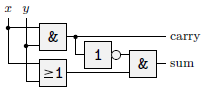
\includegraphics{halbaddierer_01}
  \end{minipage}
\end{figure}

\begin{figure}[H]
  \begin{minipage}[t]{.45\textwidth}
    Verknüpfung der beiden Funktionen erlaubt eine Implementierung mit weniger Gattern:
    $$s = (x \wedge \overline{(x \wedge y)} \vee (y \wedge \overline{(x \wedge y)}))$$
    \begin{center}
      \small (Ableitbar über Axiome)
    \end{center}
  \end{minipage}
  \hfill
  \begin{minipage}[t]{.45\textwidth}
    \caption{Halbaddierer mit weniger Gattern}
    \centering
    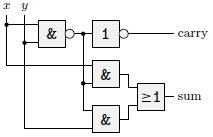
\includegraphics{halbaddierer_02}
  \end{minipage}
\end{figure}

\begin{figure}[H]
  \begin{minipage}[t]{.45\textwidth}
    Durch weiteres Ausnutzen der Booleschen Gesetze zur Vereinfachung und
    durch Nutzung anderer, zusammengesetzter Gatter ergibt sich dann eine deutlich kleinere Schaltung:
    \begin{align*}
      \centering
      s 
       & = (x \wedge \overline{y}) \vee (\overline{x} \wedge y) \\
       & = x \oplus y                                           \\
    \end{align*}
  \end{minipage}
  \hfill
  \begin{minipage}[t]{.45\textwidth}
    \caption{Optimierter Halbaddierer}
    \centering
    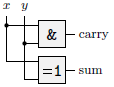
\includegraphics[scale=1.3]{halbaddierer_optimiert}
  \end{minipage}
\end{figure}


\subsection{Volladdierer}
\begin{figure}[H]
  \begin{minipage}[t]{.45\textwidth}
    Um Addition nicht nur für ein Bit, sondern für $n$ Bits, $n\geq2$, zu implementieren,
    braucht man einen

    \par \textit{Addierer mit drei Eingängen}:

    Ein Volladdierer berücksichtigt den Übertrag einer vorangehenden Addition
  \end{minipage}
  \hfill
  \begin{minipage}[t]{.45\textwidth}
    \centering
    \begin{tabular}[t]{|LLL|LL|}
      \hline
      x & y & c_{in} & s & c_{out} \\ \hline
      0 & 0 & 0      & 0 & 0       \\
      1 & 0 & 0      & 1 & 0       \\
      0 & 1 & 0      & 1 & 0       \\
      1 & 1 & 0      & 0 & 1       \\
      0 & 0 & 1      & 1 & 0       \\
      1 & 0 & 1      & 0 & 1       \\
      0 & 1 & 1      & 0 & 1       \\
      1 & 1 & 1      & 1 & 1       \\ \hline 
    \end{tabular}

  \end{minipage}
\end{figure}

\begin{figure}[H]
  \begin{minipage}[t]{.45\textwidth}
    Ein Volladdierer berechnet die Funktion
    $$s = (x + y) +x_{in}$$
    Aus diesem Grund wird er am einfachsten aus zwei Halbaddierern zusammengesetzt (mit $z = x_{in}$)
  \end{minipage}
  \hfill
  \begin{minipage}[t]{.45\textwidth}
    \centering
    \vspace{0pt}
    \caption{Volladdierer}
    \centering
    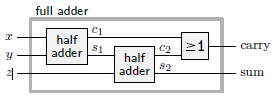
\includegraphics{volladdierer}
  \end{minipage}
\end{figure}

\subsection{n-Bit-Addierer}
\subsubsection{n-Bit-Übertragungskette-Addierer}
\begin{defbox}[Übertragungskette-Addierer]
  In einem $n$-Bit-Übertragungskette-Addierer wird mithilfe von $n$ Volladdierern Addition durchgeführt
\end{defbox}
\begin{figure}[H]
  \begin{minipage}[t]{.45\textwidth}
    ein $n$-Bit-Übertr.kette-Addierer (carry ripple adder) für $C = A + B$
    kann leicht aus $n$ Volladdierern zusammengesetzt werden\\
    \par \textit{Probleme}:
    \begin{itemize}
      \item Übertrag breitet sich wellenartig durch die Addiererkette aus
      \item Volladdierer $add_k$ kann erst anfangen, wenn $add_{k-1}$ seine Berechnung abgeschlossen hat
    \end{itemize}
  \end{minipage}
  \hfill
  \begin{minipage}[t]{.45\textwidth}
    \caption{Übertragzungskette-Addierer}
    \centering
    \vspace{0pt}
    \includegraphics[width=\textwidth]{n-bit-addierer_übertragungskette}
  \end{minipage}
\end{figure}

\subsubsection{$n$-Bit-Übertragsauswahl-Addierer}
\begin{defbox}[Übertragsauswahl-Addierer]
  In einem $n$-Bit-Übertragsauswahl-Addierer werden die Summen des unteren Halbwortes (Bits 0 bis $\frac{n}{2}-1$) und 
  des oberen Halbwortes (Bits $\frac{n}{2}-1$ bis $n$) parallel berechnet.

  Dadurch umgeht man die Problematik des wellenartigen Übertrags.
\end{defbox}

\begin{figure}[H]
  \begin{minipage}[t]{.45\textwidth}
    Da der Wert des Übertrags aus dem unteren Halbwort noch nicht bekannt ist, wenn die Summenbildung für das obere
    Halbwort beginnt, wird diese Summe zweimal, in getrennten Schaltungen berechnet:
    \begin{itemize}
      \item Schaltung 1: $c_{in} = 0$
      \item Schaltung 2: $c_{in} = 1$
    \end{itemize}
    \par Wenn der Übertrag des unteren Halbworts berechnet ist, wird er über einen 
    Multiplexer zur Auswahl des richtigen oberen Halbworts benutzt
  \end{minipage}
  \hfill
  \begin{minipage}[t]{.45\textwidth}
    \caption{Übertragungsauswahl-Addierer}
    \centering
    \includegraphics[width=\textwidth]{n-bit-addierer_übertragungsauswahl}
  \end{minipage}
\end{figure}

\begin{infobox}
  Bei längeren Binärzahlen wird das Prinzip des Übertragungsauswahl-Addierers rekusiv angewandt (d.h., die Halbwörter werden ihrerseits zerlegt)
\end{infobox}

\subsection{Darstellung negativer Zahlen}
\begin{figure}[H]
  \begin{minipage}[t]{.3\textwidth}
    \centering
    \paragraph{Betrag \& Vorzeichen}
    \small Höchstwertiges Bit gibt Vorzeichen an

    \underline{Problem}: Zahlen sollten gleiche Stellenzahl aufweisen
  \end{minipage}
  \hfill
  \begin{minipage}[t]{.3\textwidth}
    \centering
    \paragraph{Einerkomplement}
    \small Negation durch Inversion der Zahl

    \underline{Problem}: Übertrag, Zwei Darstellungen für Null
  \end{minipage}
  \hfill
  \begin{minipage}[t]{.3\textwidth}
    \centering
    \paragraph{Zweierkomplement}
    \small Negation durch Inversion und Addition von 1
  \end{minipage}
\end{figure}

\subsubsection{n-Bit-Addierer \& -Subtrahierer im Zweierkomplement}
\begin{defbox}[Addierer \& Subtrahierer im 2er-Komplement]
  $n$-Bit-Subtrahierer bestehen aus eine, $n$-Bit-Addierer und Gattern, 
  die die Negationsregel implementieren.

  \center{Idee: $A-B=A+(-B)$}
\end{defbox}

\begin{figure}[h]
  \caption{Beispiel eines n-Bit-Subtrahierers}
  \centering
  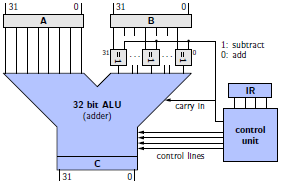
\includegraphics{n-bit-subtrahierer}
\end{figure}

\section{Multiplikation}
%TODO Binärarithmetik p37ff
\subsection{Multiplikation mit Potenzen der Basis}

\begin{figure}[H]
  \begin{minipage}[t]{0.45\textwidth}
    \paragraph{Multiplikation} mit einer Potenz der Basis $b$ des Zahlensystems ist einfach:

    Eine Multiplikation $b^k$ verschiebt die Ziffern um $k$ Stellen nach links.
    Die freiwerdenden niederwertigen Stellen werden auf $0$ gesetzt.

    \begin{alignat*}{3}
       & [d_{n-1}...d_0] &  & \cdot b^k  &  & = [d_{n-1}...d_0\ 0_1 ... 0_k]_b \\
       & 482_{10}        &  & \cdot 10^2 &  & = 48200_{10}                     \\
       & 10101_2         &  & \cdot 2^3  &  & = 10101000_2
    \end{alignat*}
  \end{minipage}
  \hfill
  \begin{minipage}[t]{0.45\textwidth}
    \paragraph{Division} durch eine Potenz der Basis $b$ ist analog zur Multiplikation:

    Eine Division durch $b^k$ verschiebt die Ziffern um $k$ Stellen nach rechts.
    Dies liefert allerdings nur den ganzzahligen Teil der Division

    \begin{alignat*}{3}
       & [d_{n-1}...d_0] &  & \div b^k  &  & = [d_{n-1}...d_k]_b \\
       & 482_{10}        &  & \div 10^2 &  & = 4_{10}            \\
       & 10101_2         &  & \div 2^3  &  & = 10_2
    \end{alignat*}
  \end{minipage}
\end{figure}


Der Rest einer Division (modulo) durch $b^k$ sind die letzten $k$ Stellen der Zahl:

\begin{alignat*}{3}
   & [d_{n-1}...d_0] &  & \ mod\ b^k  &  & = [d_{k-1}...d_0]_b \\
   & 482_{10}        &  & \ mod\ 10^2 &  & = 82_{10}           \\
   & 10101_2         &  & \ mod\ 2^3  &  & = 101_2
\end{alignat*}


\begin{infobox}
  Man beachte, dass die Division durch $b1k$ äquivalent zur Multiplikation mit $b^{-k}$ ist.
\end{infobox}


\subsection{Standardalgorithmus}
Für die allgemeine binäre Multiplikation wird der Grundschulalgorithmus des Addierens von Stellenprodukten
im Binärsystem angewandt. Die Stellenprodukte werden durch Bit-Schieben berechnet
\begin{figure}[H]
  \begin{minipage}[t]{0.45\textwidth}
    Ist die k-te Stelle des Factors $A$ eins ($A_k = 1$), so wird der Factor $B$, 
    multipliziert mit dem Stellenwert $2^k$ auf das Ergebnis aufaddiert.

    Die Multiplikation mit $2^k$ wird durch Bit-Schieben erreicht.

    Somit wird Faktor A in eine Summe von Zweierpotenzen zerlegt:
    $$A_2 = a_3 \cdot 2^3 + a_2 \cdot 2^2 + a_1  \cdot 2^1 + a_0  \cdot 2^0 $$

    \begin{table}[H]
      \begin{tabular}{LLLLLLLLL|LL}
               &   &   &   &   & 1 & 1 & 0 & 1 &   & (13)_{10}  \\
        \times &   &   &   &   & 1 & 0 & 1 & 0 &   & (10)_{10}  \\ \hline
               &   &   &   &   & 1 & 0 & 1 & 0 & 1 & (10)_{10}  \\
        +      &   &   &   & 0 & 0 & 0 & 0 &   & 0 & (0)_{10}   \\
        +      &   &   & 1 & 0 & 1 & 0 &   &   & 1 & (40)_{10}  \\
        +      &   & 1 & 0 & 1 & 0 &   &   &   & 1 & (80)_{10}  \\ \hline
        =      & 1 & 0 & 0 & 0 & 0 & 0 & 1 & 0 &   & (130)_{10}
      \end{tabular}
    \end{table}

    \par Beachte: Allgemein liefert die Multiplikation zweier $n$-Bit-Uahlen ein $2n$-Bit-Ergebnis
  \end{minipage}
  \hfill
  \begin{minipage}[t]{0.45\textwidth}
    \caption{Standardalgorithmus}
    \label{fig:standard-multiplikationsalgorithmus}
    \centering
    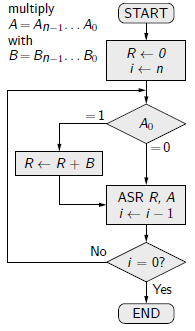
\includegraphics{standard-multiplikationsalgorithmus}
  \end{minipage}
\end{figure}

\subsection{Negative Zahlen}
Um mit den Standardalgorithmus auch Negative Zahlen multiplizieren zu können, müssen die
Faktoren auf $8$-Bit erweitert werden (aktuell $4$-Bit).

Um eine im Zweierkomplement interpretierte Zahl von $n$ auf $m$ Bit ($m>n$) zu erweitern,
müssen höherwertige Stellen passend aufgefüllt werden:

Die neuen $m-n$ Stellen bekommen den \textit{Wert des Vorzeichenbits}:

$$-4_{10} = [1\ 011]_{2k} = [1111\ 1011]_{2k} = -5_{10}$$

$$[a_{n-1} a_{n-2} a_{n-3} a_{n-4}]_{2k} = [a_{n-1} a_{n-1} a_{n-1} a_{n-1}\ a_{n-1} ... a_{n-4}]_{2k}$$

Leider reicht die Stellenerweiterung alleine nicht immer aus, faher ist es angebracht eine andere Methode zu suchen,
die mit negativen Zahlen besser umgehen kann: \textit{Booths Algorithmus}

\subsection{Booths Algorithmus}
\begin{defbox}[Booths Algorithmus]
  Die Kernidee von Booths Algorithmus ist es, den ersten Faktor im Produkt $a \cdot b$ in der Form:
  $$a = (a_1 - a_2) + (a_3 - a_4) + ... + (a_{k-1} - a_k)$$
  zu zerlegen, so dass die Multiplikation $a \cdot b$ zu:
  $$a \cdot b = a_1b - a_2b + a_3b - a_4b + ... + a_{k-1}b - a_kb$$

  Dies ist nützlich, da eine Differenz von Zweierpotenzen einer Binärzahl mit genau einer Kette von Einsen entspricht.
  Dementsprechend benötigt der Algorithmus nur so viele Additionen, wie es Wechsel zwischen 1 und 0 (und umgekehrt 0 und 1) im Faktor A gibt.

  \begin{align*}
    7_{10} = 00000111_2 = 1000_2 - 0001_2 = 2^3_{10} - 2^0_{10}
  \end{align*}
\end{defbox}


\begin{figure}[H]
  \begin{minipage}[t]{0.6\textwidth}
    \begin{table}[H]
      \small
      \centering
      \begin{tabular}{LLLLLLLLL|LLL}
               & {\color[HTML]{9B9B9B} 0} & {\color[HTML]{9B9B9B} 0} & {\color[HTML]{9B9B9B} 0} & {\color[HTML]{9B9B9B} 0} & 0                        & 1                        & 1                        & 1                        &   & (+7)_{10}  & B                         \\
        \times & {\color[HTML]{9B9B9B} 1} & {\color[HTML]{9B9B9B} 1} & {\color[HTML]{9B9B9B} 1} & {\color[HTML]{FFCB2F} 1} & {\color[HTML]{FE0000} 1} & {\color[HTML]{FE0000} 0} & {\color[HTML]{FE0000} 1} & {\color[HTML]{FE0000} 1} &   & (-5)_{10}  & A                         \\ \hline
        +      & 0                        & 0                        & 0                        & 0                        & 0                        & 1                        & 0                        & 1                        & 1 & (5)_{10}   & -2^0 \cdot B              \\
        +      & 0                        & 0                        & 0                        & 0                        & 0                        & 0                        & 0                        & {\color[HTML]{9B9B9B} 0} & 1 & (0)_{10}   &                           \\
        +      & 0                        & 0                        &                          & 0                        & 0                        & 0                        & {\color[HTML]{9B9B9B} 0} & {\color[HTML]{9B9B9B} 0} & 1 & (0)_{10}   &                           \\
        +      & {\color[HTML]{FFCB2F} 1} & {\color[HTML]{FE0000} 1} & {\color[HTML]{FE0000} 0} & {\color[HTML]{FE0000} 1} & {\color[HTML]{FE0000} 1} & {\color[HTML]{9B9B9B} 0} & {\color[HTML]{9B9B9B} 0} & {\color[HTML]{9B9B9B} 0} & 1 & (-40)_{10} & 2^3 \cdot B               \\ \hline
        =      & 1                        & 1                        & 0                        & 1                        & 1                        & 1                        & 0                        & 1                        &   & (-35)_{10} & 2^3 \cdot B - 2^0 \cdot B
      \end{tabular}
    \end{table}

    Wir haben hier $7_{10}$ in $7_{10} = 8_{10}-1_{10} = 2^3_{10} - 2^0_{10} = 1000_2 - 0001_2$ zerlegt

  \end{minipage}
  \hfill
  \begin{minipage}[t]{0.3\textwidth}
    \caption{Booths Algorithmus}
    \label{fig:booths-multiplikationsalgorithmus}
    \begin{center}
      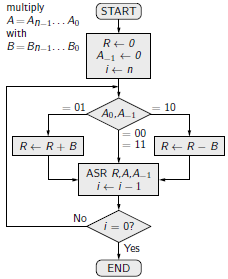
\includegraphics[width=\textwidth]{booths-multiplikationsalgorithmus}
    \end{center}
  \end{minipage}
\end{figure}

\paragraph{Negativer erster Faktor:}

Im Fall, dass der erste Faktor negativ ist, es also eine 1 als Vorzeichen gibt, dann können die führenden einsen ignoriert werden:

\begin{alignat*}{3}
  11111011_2 
   & = 11111111_2          & + & (10000000_2 - 1000_2)           & + & (0100_2 - 0001_2)     \\
   & = -2^7_{10}           & + & (2^7_{10} - 2^3_{10})           & + & (2^2_{10} - 2^0_{10}) \\
   & = \bcancel{-2^7_{10}} & + & (\bcancel{2^7_{10}} - 2^3_{10}) & + & (2^2_{10} - 2^0_{10}) \\
   & =   \                 & - & 2^3_{10}                        & + & 2^2_{10} - 2^0_{10}
\end{alignat*}


\section{Die Arithmetisch-Logische-Einheit (Arithmetic Logical Unit. ALU)}
\subsection{Die ALU in der Hack-Architektur}
\begin{figure}[H]
  \begin{minipage}[t]{0.5\textwidth}
    Die Eingaben $zx$, $nx$, $ny$, $f$ und $no$ kodieren die auszuführende Operation:

    \begin{table}[H]
      \begin{tabular}{Cl}
        zx   & Setze Eingabe $x=0$                        \\
        $zy$ & Setze Eingabe $y=0$                        \\
        $nx$ & Bilde Einerkomplement der Eingabe $x$      \\
        $ny$ & Bilde Einerkomplement der Eingabe $y$      \\
        $f$  & Wählt Operation: Addition / bitweises Und  \\
        $no$ & Bilde Einerkomplement der Ausgabe $out$    \\
        $zr$ & Zero Flag ($zr=1 \rightarrow out = 0$)     \\
        $ng$ & Negative Flag ($ng=1 \rightarrow out < 0$)
      \end{tabular}
    \end{table}

    Über-/Unterlauf wird ignoriert
  \end{minipage}
  \hfill
  \begin{minipage}[t]{0.4\textwidth}
    \caption{ALU - Hack (16 Bit)}
    \label{fig:alu_der_hack-platform}
    \centering
    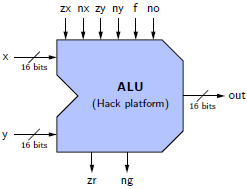
\includegraphics[width=\textwidth]{alu_der_hack-platform}
  \end{minipage}
\end{figure}

Durch die 6 Steuerbits (Abb. \ref{fig:alu_der_hack-platform}) kann im Prinzip zwischen 
$2^6=62$ Wahrheitstafeln ausgewählt werden, von diesen sind allerdings nur 18 relevant.

\begin{defbox}
  \begin{figure}[H]
    \begin{minipage}[t]{0.45\textwidth}
      Die Steuerbits dienen als Eingaben für Steuergatter, die zugeordneten
      Operationen bewirken.

      Diese Steuergatter können, wie in Abb. \ref{fig:alu_steuerbits} die Eingabe oder,
      wie im Fall von $no$ die Ausgabe verändern.
    \end{minipage}
    \hfill
    \begin{minipage}[t]{0.45\textwidth}
      \caption{CAPTION}
      \label{fig:alu_steuerbits}
      \centering
      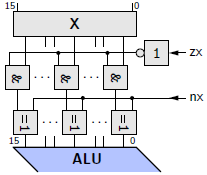
\includegraphics{alu_steuerbits}
    \end{minipage}
  \end{figure}
\end{defbox}


\begin{table}[H]
  \caption{Funktionen der ALU auf der Hack-Plattform}
  \label{tbl:alu_funktionen}
  \centering
  \begin{tabular}{|C|C|C|C|C|C|C|}
    \hline
    \multicolumn{2}{|c|}{\begin{tabular}[c]{@{}c@{}}Voreinstellung \\ für Eingabe x\end{tabular}} & \multicolumn{2}{c|}{\begin{tabular}[c]{@{}c@{}}Voreinstellung \\ für Eingabe y\end{tabular}} & \begin{tabular}[c]{@{}c@{}}Einstellung für \\ Addition (+) \\ und \\ bitw. Und ( \& )\end{tabular} & \begin{tabular}[c]{@{}c@{}}Einstellung \\ für Output \end{tabular} & \text{ALU Output}                                                  \\ \hline
    zx                                               & nx                                              & zy                         & ny                         & f                                          & no         & out      \\ \hline
    zx                                               & nx                                              & zy                         & ny                         &                                            & no         &          \\
    \downarrow                                       & \downarrow                                      & \downarrow                 & \downarrow                 & f   \rightarrow out = x + y                & \downarrow & f(x,y)   \\
    x = 0                                            & x = -x                                          & y = 0                      & y = -y                     & \overline{f} \rightarrow out = x \ \&\   y & out = -out &          \\ \hline
    1                                                & 0                                               & 1                          & 0                          & 1                                          & 0          & 0        \\
    1                                                & 1                                               & 1                          & 1                          & 1                                          & 1          & 1        \\
    1                                                & 1                                               & 1                          & 0                          & 1                                          & 0          & -1       \\
    0                                                & 0                                               & 1                          & 1                          & 0                                          & 0          & x        \\
    1                                                & 1                                               & 0                          & 0                          & 0                                          & 0          & y        \\
    0                                                & 0                                               & 1                          & 1                          & 0                                          & 1          & ~x       \\
    1                                                & 1                                               & 0                          & 0                          & 0                                          & 1          & ~y       \\
    0                                                & 0                                               & 1                          & 1                          & 1                                          & 1          & -x       \\
    1                                                & 1                                               & 0                          & 0                          & 1                                          & 1          & -y       \\
    0                                                & 1                                               & 1                          & 1                          & 1                                          & 1          & x+1      \\
    1                                                & 1                                               & 0                          & 1                          & 1                                          & 1          & y+1      \\
    0                                                & 0                                               & 1                          & 1                          & 1                                          & 0          & x-1      \\
    1                                                & 1                                               & 0                          & 0                          & 1                                          & 0          & y-1      \\
    0                                                & 0                                               & 0                          & 0                          & 1                                          & 0          & x+y      \\
    0                                                & 1                                               & 0                          & 0                          & 1                                          & 1          & x-y      \\
    0                                                & 0                                               & 0                          & 1                          & 1                                          & 1          & y-x      \\
    0                                                & 0                                               & 0                          & 0                          & 0                                          & 0          & x\ \&\ y \\
    0                                                & 1                                               & 0                          & 1                          & 0                                          & 1          & x\ |\ y  \\ \hline
  \end{tabular}
\end{table}
\subsection{Einbindung der ALU in den Prozessor der Hack-Architektur}


\chapter{Sequentielle Logik}
\section{Sequentielle Logik}
\subsection{Logikschaltungen: Kombinatorische \& Sequentielle Logik}
\begin{figure}[H]
  \begin{minipage}[t]{0.48\textwidth}
    \paragraph{Kombinatorische Logik}

    \centering

    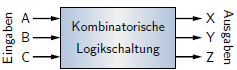
\includegraphics[width=\textwidth]{kombinatorische_logik}

  \end{minipage}
  \hfill
  \begin{minipage}[t]{0.48\textwidth}
    \paragraph{Sequentielle Logik}

    \centering

    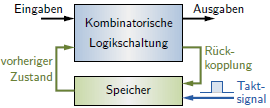
\includegraphics[width=\textwidth]{sequentielle_logik}
  \end{minipage}
\end{figure}

\begin{figure}[H]
  \begin{minipage}[t]{0.48\textwidth}
    \centering
    \underline{Implementierung: Schaltnetze}

    \begin{itemize}
      \item Einfaches Berechnen von Ein- \& Ausgaben
      \item Keine Informationsspeicherung
      \item Zustandslosigkeit
      \item verzögerungsfreie Berechnung
    \end{itemize}
  \end{minipage}
  \hfill
  \begin{minipage}[t]{0.48\textwidth}
    \centering
    \underline{Implementierung: Schaltwerke}

    \begin{itemize}
      \item Rückkopplung von Ausgaben auf Eingaben
      \item Explizite Informationsspeicherung
      \item Unterscheidung von Zuständen
      \item Gatterlaufzeiten explizit berücksichtigt
    \end{itemize}

  \end{minipage}
\end{figure}

\begin{figure}[H]
  \begin{minipage}[t]{0.45\textwidth}
    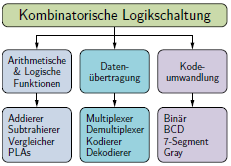
\includegraphics[width=\textwidth]{kombinatorische_logikschaltung}
  \end{minipage}
  \hfill
  \begin{minipage}[t]{0.45\textwidth}
    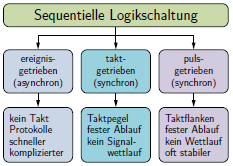
\includegraphics[width=\textwidth]{sequentielle_logikschaltung}
  \end{minipage}
\end{figure}

\subsection{Prinzip der Rückkopplung}
\begin{defbox}[Rückkopplung]
  \begin{figure}[H]
    \begin{minipage}[t]{0.7\textwidth}
      Durch Rückkopplung werden Ausgaben als Eingabesignal verwendet. 
      Hierdurch kann ein (Ausgabe-) Zustand festgehalten werden, 
      bis ein Ergeignis ihn wieder ändert.
    \end{minipage}
    \hfill
    \begin{minipage}[t]{0.25\textwidth}
      \includegraphics{rückgekoppelter_2_wege_multiplexer}
    \end{minipage}
  \end{figure}
\end{defbox}

\paragraph{Probleme der Rückkopplung}

Durch Rückkopplung kann es zu (unerwünschten) \textit{Schwingungen} kommen. 
Diese sind ein Beispiel für \textit{Signallaufzeitprobleme}, die durch Rückkopplungen auftreten können).

Ein weiteres Beispiel sind sogenannte \textit{Wettlaufsituationen (Race Conditions)}, die auftreten, 
wenn sich zwei Signale auf zwei oder mehr Wegen ausbreiten, und die Ausgabe davon abhängen kann, 
welches Signal schneller weitergegeben wird

Signallaufzeitprobleme lassen sich am leichtesten durch ein zentral erzeugtes \underline{\textit{Taktsignal}} vermeiden, 
das bestimmt, wann Eingaben übernommen werden.

\subsection{Asynchrone und synchrone Schaltwerke}

\begin{figure}[H]
  \begin{minipage}[t]{0.45\textwidth}
    \centering
    \paragraph{Asynchrone Schaltwerke}
    \begin{itemize}
      \item Direkte Steuerung durch Änderung der Eingangssignale
      \item Wann und ob ein stabiler Zustand erreicht wird von Gatterlaufzeit abhängig
      \item Oft komplizierter, aufwendiger Entwurf
      \item Sehr schnelle Schaltwerke möglich
    \end{itemize}
  \end{minipage}
  \hfill
  \begin{minipage}[t]{0.45\textwidth}
    \centering
    \paragraph{Synchrone Schaltwerke}
    \begin{itemize}
      \item Steuerung durch Taktsignal
      \item Eingangssignale nur zu von Takt festgelegten Zeitpunkten übernommen
      \item Meist einfacher, systematischer Entwurf.
      \item Langsamstes Bauteil bestimmt maximal mögliche Taktfrequenz
    \end{itemize}
  \end{minipage}
\end{figure}

\subsection{Taktsignal (Clock Signal)}
\begin{defbox}
  Ein \textit{Taktsignal} (Clock Signal) wird meist durch einen \textit{Quarzoszillator} erzeugt. 
  Durch elektromagnetische Resonanz eines pezoelektrischen Quarzkristalls (Schwingquarz)
  entsteht ein Taktsignal mit fester Frequenz.
\end{defbox}




\begin{figure}[H]
  \begin{minipage}[t]{0.45\textwidth}
    \paragraph{Taktzyklus / -periode (Cycle / Period)} $T$:
    \par Zeit zwischen steigenden/fallenden Flanke und der nächsten\\

    \paragraph{Taktfrequenz (Frequency)} $f$:
    \par Reziprokwert der Taktperiode $T$\\

    \paragraph{Taktbreite (Width)}:
    \par Die Zeit zwischen einer steigenden und fallenden Flanke 
    (kann aber muss nicht die Hälfte der Taktperiode sein)\\

    \paragraph{Taktpegel / Taktzustand}:
    \par 1-Pegel (Versorgungsspannung, high) und 0-Pegel (Masse, low) - 
    Unterscheidung der Phasen im Taktzyklus\\

  \end{minipage}
  \hfill
  \begin{minipage}[t]{0.45\textwidth}
    \caption{Idealisierend: Taktsignal als Folge von Rechteckimpulsen}
    \begin{center}
      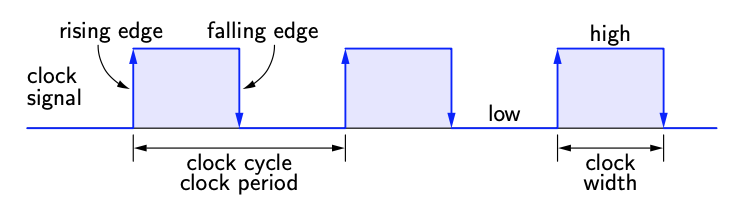
\includegraphics[width=\textwidth]{taktsignal_01}
    \end{center}

    \begin{center}
      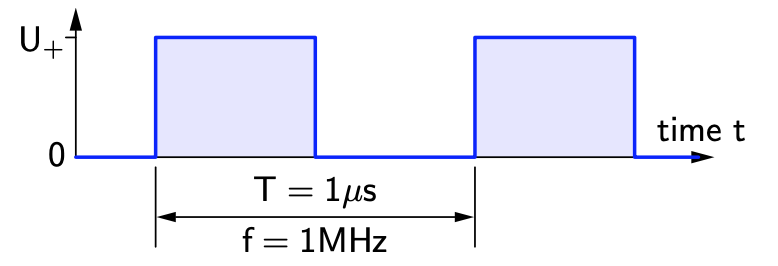
\includegraphics[width=\textwidth]{taktsignal_02}
    \end{center}
  \end{minipage}
\end{figure}

\begin{infobox}
  \begin{itemize}
    \item Oft ist die Reihenfolge von Berechnungen wichtig (manche können parallel, andere müssen strikt sequentiell abgearbeitet werden)
          \par $\rightarrow$ Das Taktsignal gilt als \"Zeitgeber\" für solche Berechnungen.
    \item Typische Taktfrequenzen liegen im zwischen einigen KiloHertz (kHz) und einigen GigaHertz (GHz)
    \item Manchmal werden asymmetrische Taktsignale benötigt, die durch Verzögerung (delay) und logische Und-Verknüpfung mit dem Original erzeugt werden
          \begin{figure}[H]
            \begin{minipage}[t]{0.45\textwidth}
              \caption{Erzeugung eines verzögerten Taktsignals}
              \begin{center}
                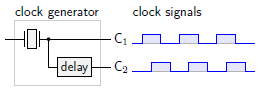
\includegraphics{taktsignal_asymmetrisch}
              \end{center}
            \end{minipage}
            \hfill
            \begin{minipage}[t]{0.45\textwidth}
              \caption{Asym. Taktsignal durch Und-Verknüpfung}
              \begin{center}
                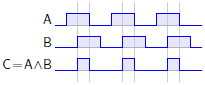
\includegraphics{taktsignal_asymmetrisch_02}
              \end{center}
            \end{minipage}
          \end{figure}
  \end{itemize}
\end{infobox}


\section{Bistabile Kippstufen}
\begin{defbox}
  Eine \textit{bistabile Kippstufe}, auch \textit{bistabiles Kippglied} oder \textit{Riegel},
  ist eine rückgekoppelte Schaltung aus zwei NOR- oder zwei NAND-Gattern mit zwei Ein- und Ausgängen 
  (auch speziell \textit{SR-Riegel} genannt), die zwei Stabile (daher bistabile) und einen metastabilen Zusstand hat.

  \par Oft wird einfach (aber ungenau) von \textit{FlipFlop} gesprochen
\end{defbox}
\begin{figure}[H]
  \caption{Übersicht: Bistabile Kippstufen}
  \centering
  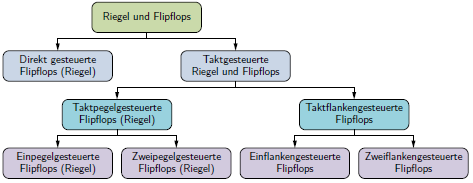
\includegraphics{kippstufen_zusammenfassung}
\end{figure}


\subsection{Implementierung mit Gattern}

\begin{figure}[H]
  \begin{minipage}[t]{0.45\textwidth}
    \caption{Riegel aus NOR-Gattern}
    \centering
    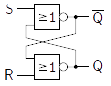
\includegraphics{riegel_nor}
  \end{minipage}
  \hfill
  \begin{minipage}[t]{0.45\textwidth}
    \caption{Riegel aus NAND-Gattern}
    \centering
    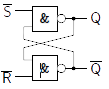
\includegraphics{riegel_nand}
  \end{minipage}
\end{figure}

\begin{figure}[H]
  \caption{Zusammenfassung aller Zustände bistabiler Kippstufen}
  \centering
  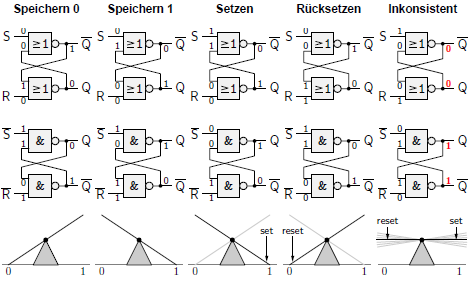
\includegraphics[width=0.8\textwidth]{riegel_zusammenfassung}
\end{figure}

\subsection{SR-Riegel}

\subsubsection{Stabile Zustände}
Wenn die Eingabe des Riegels $S=R=0$ (bzw. $\overline{S}=\overline{R}=1$ im NAND-Gatter) ist, bleibt der Riegel stabil $0$ oder $1$:

\begin{figure}[H]
  \begin{minipage}[t]{0.48\textwidth}
    \caption{NOR-Riegel mit $S=R=0$}
    \centering
    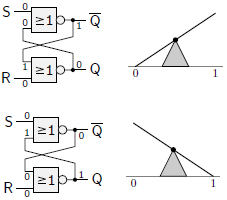
\includegraphics{riegel_nor_stabil}
  \end{minipage}
  \hfill
  \begin{minipage}[t]{0.48\textwidth}
    \caption{NAND-Riegel mit $\overline{S}=\overline{R}=1$}
    \centering
    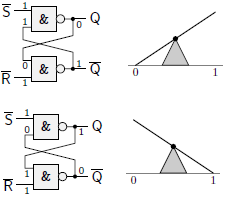
\includegraphics{riegel_nand_stabil}
  \end{minipage}
\end{figure}

Die Eingabe kann somit als \textit{Speicherzustand} interpretiert werden, 
in dem die Kippstufe ihren Zustand beibehält

\subsubsection{Setzen \& Rücksetzen (set \& reset)}

\begin{figure}[H]
  \begin{minipage}[t]{0.45\textwidth}
    \centering
    Die Eingabe

    $S=1, R=0$ (NAND: $\overline{S} = 0,\ \overline{R} = 1$)

    kann als Setzen (set) interpretiert werden \\ \ 
  \end{minipage}
  \hfill
  \begin{minipage}[t]{0.45\textwidth}
    \centering
    Die Eingabe 

    $S=0, R=1$ (NAND: $\overline{S} = 1,\ \overline{R} = 0$) 

    kann als Rücksetzen (reset) interpretiert werden
  \end{minipage}
\end{figure}


\begin{figure}[H]
  \begin{minipage}[t]{0.48\textwidth}
    \caption{NOR-Riegel}
    \centering
    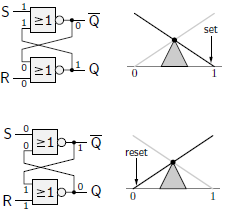
\includegraphics{riegel_nor_set_reset}
  \end{minipage}
  \hfill
  \begin{minipage}[t]{0.48\textwidth}
    \caption{NAND-Riegel}
    \centering
    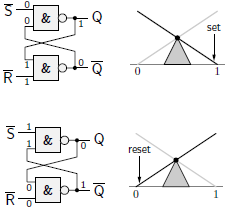
\includegraphics{riegel_nand_set_reset}
  \end{minipage}
\end{figure}

Diese Zustände bleiben erhalten, wenn die Eingaben auf $S=R=0$ (NAND: $\overline{S} = \overline{R} = 1)$ wechseln.

\subsubsection{Inkonsistenter (metastabiler) Zustand}
Die Eingaben $S=R=1$ (NAND: $\overline{S}=\overline{R}=0$) führen zu einem inkonsistenten Zustand,
da in diesem Fall $Q=\overline{Q}=0$ (NAND: $Q=\overline{Q}=1$) gilt,
also die Ausgänge nicht komplementär sind,
ausserdem der Übergang in den Speicherzustand $S=\overline{R}=0$ (NAND: $\overline{A}=\overline{\overline{R}}=1$) undefiniert ist.

\begin{figure}[H]
  \begin{minipage}[t]{0.48\textwidth}
    \caption{NOR-Riegel}
    \centering
    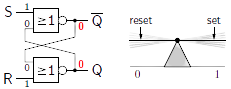
\includegraphics{riegel_nor_inconsistent}
  \end{minipage}
  \hfill
  \begin{minipage}[t]{0.48\textwidth}
    \caption{NAND-Riegel}
    \centering
    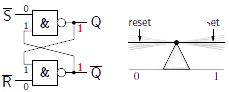
\includegraphics{riegel_nand_inconsistent}
  \end{minipage}
\end{figure}

Dieser Zustand wird \underline{metastabil} genannt, da der Speicherzustand undefiniert wird.
Die Kippstufe bleibt in diesem Zustand, bis eine Eingabe die Oberhand gewinnt und sie in den zugehörigen Zustand bringt.

\begin{infobox}
  Bistabile Kippstufen können durch ihre beiden stabilen Zustände ein Bit speichern,
  aber der metastabile Zustand ist problematisch.

\end{infobox}

\begin{exbox}[Anwendung - Prellfreier Schalter/Taster]
  Bei elektromagnetischen Schaltern kommt es durch mechanische Störeffekte oft zu einem sogenannten Prellen des Schalters.
  Statt eines sofortigen Schaltensch, kommt es kurzzeitig zu mehrfachem.

  \par Wird an die Schalterkontakte eine bistabile Kippstufe angeschlossen, so wird das Prellen unterdrückt,
  da ein mehrfaches Eingangssignal nur einmalig zu einer Zustandsänderung führt.
  \begin{figure}[H]
    \begin{minipage}[t]{0.45\textwidth}
      \centering
      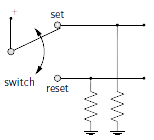
\includegraphics{riegel_prellender_schalter}
    \end{minipage}
    \hfill
    \begin{minipage}[t]{0.45\textwidth}
      \centering
      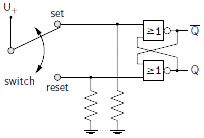
\includegraphics{riegel_prellfreier_schalter}
    \end{minipage}
  \end{figure}
\end{exbox}

\subsection{Direkt gesteuerte FlipFlops (Riegel)}
Durch vorgeschaltete Zusatzgitter kann die problematische Eingabe $S=R=1$ bzw. $\overline{S} = \overline{R}=0$ ausgeschlossen werden.
\subsubsection{D-Riegel (D latch)}
\begin{figure}[H]
  \begin{minipage}[t]{0.45\textwidth}
    \begin{itemize}
      \item Stellt sicher, dass $R = \neg S$
      \item Vorteil: Schließt problematische Eingaben aus
      \item Nachteil: $S=R=0$ geht ebenfalls verloren
    \end{itemize}
  \end{minipage}
  \hfill
  \begin{minipage}[t]{0.45\textwidth}
    \caption{D-Riegel}
    \centering
    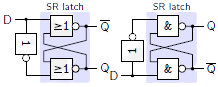
\includegraphics{riegel_d-riegel}
  \end{minipage}
\end{figure}


\subsubsection{E-Riegel (E latch)}
\begin{figure}[H]
  \begin{minipage}[t]{0.45\textwidth}
    \begin{itemize}
      \item Stellt sicher, dass $R = \neg S$
      \item Vorteil: Schließt problematische Eingaben aus
      \item Nachteil: $S=R=0$ geht ebenfalls verloren
      \item Man beachte, dass die NAND-Form keine negierten Eingaben mehr hat!
    \end{itemize}
  \end{minipage}
  \hfill
  \begin{minipage}[t]{0.45\textwidth}
    \caption{E-Riegel}
    \centering
    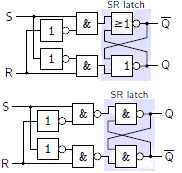
\includegraphics{riegel_e-riegel}
  \end{minipage}
\end{figure}

\subsection{Taktpegelsteuerung}
Durch anlegen eines Taktsignals, können Riegel ihre Eingaben bedingt sperren, so dass nur bei 1-Taktpegel Eingaben übernommen werden.
\begin{figure}[H]
  \begin{minipage}[t]{0.45\textwidth}
    \begin{itemize}
      \item Sperrt Eingaben bedingt, so dass $S=R=1$ im Sperrzustand keinen Schaden mehr anrichten kann
      \item Man beachte, dass die NAND-Form keine negierten Eingaben mehr hat!
    \end{itemize}

    Zusätzliches Sicherstellen von $R = \neg S$ ergibt den \textit{sperrbaren D-Riegel}:
    \begin{figure}[H]
      \caption{Sperrbarer D-Riegel}
      \centering
      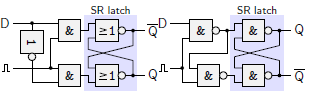
\includegraphics{riegel_sperrbarer-d-riegel}
    \end{figure}
  \end{minipage}
  \hfill
  \begin{minipage}[t]{0.45\textwidth}
    \caption{Sperrbarer SR-Riegel}
    \centering
    \vspace{0px}
    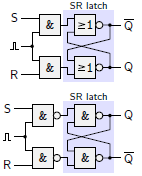
\includegraphics{riegel_sperrbarer-sr-riegel}
  \end{minipage}
\end{figure}

\subsection{Taktpegelsteuerung mit Rückkopplung}
Durch eine Rückkopplung der Ausgaben des SR-Riegels auf die Sperrgatter lässt sich erreichen, 
dass die Eingabe $S=R=1$ eine neue Funktion erhält:

Das Umkehren (toggle) des bestehenden Speicherzustands

\begin{figure}[H]
  \begin{minipage}[t]{0.45\textwidth}
    \subsubsection{T-Riegel (T latch)}
    \centering    
    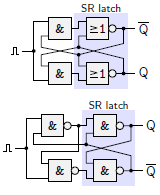
\includegraphics{riegel_t-riegel}
  \end{minipage}
  \hfill
  \begin{minipage}[t]{0.45\textwidth}
    \subsubsection{JK-Riegel (JK latch)}
    \centering    
    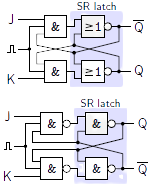
\includegraphics{riegel_jk-riegel}
  \end{minipage}
\end{figure}

\begin{warnbox}[Laufzeitprobleme (Schwingungen)]
  Man beach   te aber: Das durch die Eingabe $S=R=1$ bewirkte Umkehren führt 
  zu Laufzeitproblemen (Schwingungen), da sich kein stabiler Zustand einstellt
\end{warnbox}


\subsection{Taktflankensteuerung}
Problem der Taktpegelsteuerung ist, dass die Eingaben während der gesamten 1-Phase des Taktes eine Wirkung auf den Zustand des Riegels ausüben.

Besser wäre eine Übernahme der Eingaben an der steigenden Flanke: Die Taktflankensteuerung

\begin{defbox}[Taktflankensteuerung]
  Taktflankensteuerung löst das Problem der Taktpegelsteuerung, bei dem die Eingaben 
  während der gesamten 1-Phase des Taktes eine Wirkung auf den Zustand des Riegels ausüben.

  Bei Taktflankensteuerung spricht man nicht mehr von Riegel (dieser ist direkt oder taktpegelgesteuert), sondern von \textit{FlipFlop}
\end{defbox}

\begin{figure}[H]
  \begin{minipage}[t]{0.45\textwidth}
    Durch die Nutzung von NOT-Gattern (Invertern) können Signale verzögert werden (Verzögerungsglieder).

    Verbindet man diese mit einem AND-Gatter, bilden sie ein \textit{Impulsglied}

    Dadurch wird aus einer Taktflanke ein kurzer \textit{Taktimpuls} erzeugt
  \end{minipage}
  \hfill
  \begin{minipage}[t]{0.45\textwidth}
    \caption{Schaltung zur Erzeugung eines Taktimpulses}
    \centering
    \includegraphics{taktflankensteuerung_verzögerungsglieder}
    \includegraphics{taktflankensteuerung_laufzeit}
  \end{minipage}
\end{figure}

Zur Implementierung der Taktflankensteuerung schaltet man eine Schaltung (wie oben) vor 
den Eingang für das Taktsignal.

\begin{figure}[H]
  \begin{minipage}[t]{0.45\textwidth}
    \caption{D-FlipFlop (D-Riegel mit Taktflankensteuerung)}
    \centering
    \includegraphics{taktflankensteuerung_d-flipflop}
  \end{minipage}
  \hfill
  \begin{minipage}[t]{0.45\textwidth}
    \caption{JK-FlipFlop (JK-Riegel mit Taktflankensteuerung)}
    \centering
    \includegraphics{taktflankensteuerung_jk-flipflop}
  \end{minipage}
\end{figure}

\begin{infobox}[Taktflankensteuerung \& Laufzeitprobleme]
  Taktflankensteuerung mindert Laufzeitprobleme und macht Schaltungen robuster, da Gatterlaufzeiten von den Umgebungsbedingungen abhängen können,
  kann es aber dennoch zu Laufzeitproblemen kommen.
\end{infobox}

\subsection{Master-Slave-Prinzip}
Gerade hintereinandergeschaltete FlipFlops können noch zu Problemen führen,
wenn eine vorangehende Stufe schon ihre Ausgaben ändert,
bevor die nachfolgende Stufe die Eingabeauswertung abgeschaltet hat. (Gatterlaufzeiten!)

\begin{defbox}
  Beim \textit{Master-Slace-Prinzip} werden zwei Riegel hintereinandergeschaltet. 
  Der erste (vordere) Riegel (Master) wertet seine Eingaben während des 1-Taktpegels, 
  der zweite (hintere) Riegel (Slave) wertet seine Eingaben während des 0-Taktpegels aus.

  Während der eine Riegel seine Ausgaben auswertet, sind die Ausgaben des jeweils anderen stabil,
  da jeweils nur einer der Riegel aktiv ist.

  So kann man (fast) alle Laufzeitprobleme vermeiden
\end{defbox}

Implementiert wird das Prinzp mit \textit{Zweipegelsteuerung}. Hierbei bekommt der Slave-riegel
ein Taktsignal, das gegenüber dem Master-Riegel invertiert ist.

\subsection{Schaltzeichen}
Da Riegel und Flipflops sehr häufig verwendete Schaltungsbausteine sind, werden sie durch eigene Schaltzeichen dargestellt.

Diese Schaltzeichen sind einfache Rechtecke:

\subsubsection{Ein- und Ausgänge:}
\begin{figure}[H]
  \begin{minipage}[t]{0.45\textwidth}
    \begin{itemize}
      \item Eingänge links (z.B.: S, D, J)
      \item Ausgänge rechts (z.B.: R, K)
      \item Setzen-Eingange oben, Rücksetzen-Eingang unteren
      \item Ausgang $Q$ oben, $\overline{Q}$ unten.
      \item Negationszeichen am Ausgang $\overline{Q}$
      \item Setzen- und Rücksetzen-Eingänge: 1 links der Bezeichnung versehen (z.B.: 1S, 1R, 1D, 1J, 1K)
    \end{itemize}
  \end{minipage}
  \hfill
  \begin{minipage}[t]{0.45\textwidth}
    \caption{Schaltzeichen - SR-Riegel}
    \centering
    \includegraphics[scale=1.2]{schaltzeichen}
  \end{minipage}
\end{figure}


\subsubsection{Gated- / Clock-Eingänge:}
\begin{figure}[H]
  \begin{minipage}[t]{0.45\textwidth}
    \begin{itemize}
      \item Gated (G) und Clock (C) Eingänge: links in der Mitte
      \item Eingänge, die Setzten-/Rücksetzen-Eingänge modifizieren: 1 links der Bezeichnung (z.B.: G1, C1)
      \item Negationsblase: Takteingänge mit reagieren auf 0-Taktpegel, ohne auf 1-Taktpegel (Flipflops: fallende, ohne steigende Flanke )
      \item weißes Dreieck an einem Takteingang: \textit{Taktflankensteuerung}
      \item Winkel an Ausgang: Master-Slave-Flipflops
    \end{itemize}
  \end{minipage}
  \hfill
  \begin{minipage}[t]{0.45\textwidth}
    \caption{Riegel mit Gate \& Clock \& Master-Slave}
    \centering
    \includegraphics{schaltzeichen_gate_clock_master-slave}
  \end{minipage}
\end{figure}

\subsection{Schaltverhalten}
%TODO Sequentielle Logik - p44


\section{Register, Zähler und Speicher}
\subsection{Schieberegister und Zähler}
\begin{defbox}
  Schieberegister können durch Verkettung von D-Flipflops erstellt werden.
  Mit jedem Taktzyklus wird der Speicherinhalt der Flipsflops um ein Flipsflop weitergeschoben.

  Schieberegister haben eine feste Anzahl von Speicherplätzen (Anzahl der Flipflops) und arbeiten
  nach dem FIFO-Prinzip.
\end{defbox}

\begin{figure}[H]
  \begin{minipage}[t]{0.45\textwidth}
    \caption{4-Bit seriell zu parallel}
    \label{fig:schieberegister_01}
    \centering
    \includegraphics{schieberegister_01}
  \end{minipage}
  \hfill
  \begin{minipage}[t]{0.45\textwidth}
    \caption{4-Bit parallel zu seriell}
    \label{fig:schieberegister_02}
    \centering
    \includegraphics{schieberegister_02}
  \end{minipage}
\end{figure}

Schieberegister können auch zur Wandlung eines seriellen Datenstroms in einen parallelen (\ref{fig:schieberegister_01})
oder eines parallelen Datenstroms in einen seriellen (\ref{fig:schieberegister_02}) benutzt werden.

\subsubsection{Einfache Rückgekoppelte Schieberegister: Ringzähler}
\begin{figure}[H]
  \begin{minipage}[t]{0.45\textwidth}
    \caption{Einf. 4-Bit-Ringzähler}

    \centering
    \includegraphics{4-bit-ringzähler}

    \includegraphics{4-bit-ringzähler-takt}
  \end{minipage}
  \hfill
  \begin{minipage}[t]{0.45\textwidth}
    \caption{4-Bit-Johnson-Ringzähler}

    \centering
    \includegraphics{4-bit-johnson-ringzähler}

    \includegraphics{4-bit-johnson-ringzähler-takt}
  \end{minipage}
\end{figure}

\subsubsection{Linear Rückgekoppelte Schieberegister: Ringzähler}

\begin{figure}[H]
  \begin{minipage}[t]{0.45\textwidth}
    \caption{Linear Rückgekoppeltes Schieberegister (LFSR)}
    \label{fig:lfsr}
    \includegraphics{lfsr}
  \end{minipage}
  \hfill
  \begin{minipage}[t]{0.45\textwidth}
    \caption{Linear Rückgekoppeltes Schieberegister (LFSR)}
    \label{fig:lfsr_vereinfacht}
    \includegraphics{lfsr_vereinfacht}
  \end{minipage}
\end{figure}

Durch komplizierte Rückkopplungen, die nicht nur vom letzten Flipflop, sondern auch von dazwischenliegenden
rückkoppeln (Verknüpfung der Rückkopplungen über exklusives Oder) kann man komplizierte Bitfolgen erzeugen

Solche \textit{linear rückgekoppelten Schieberegister} werden vereinfacht wie Abb. \ref{fig:lfsr_vereinfacht} dargestellt

\begin{figure}[H]
  \caption{Linear Rückgekoppeltes Schieberegister}
  \label{fig:lfsr_long}
  \centering
  \includegraphics{lfsr_long}
\end{figure}

Das LFSR in Abb. \ref{fig:lfsr_long} hat Rückkopplungen von den Positionen 10, 12, 13 und 15.
Solche Schieberegister werden z.B. zur Erzeugung von Pseudozufallszahlen oder zur Zyklischen Redundanzprüfung verwendet


\subsubsection{Zähler}
%TODO Sequentielle Logik - p54
\subsubsection{Steuerbare Zähler}

\subsection{Speicherzellen und Programmzähler}
\subsubsection{Speicherzellen \& -register}
\subsubsection{Programmzähler}


\section{Hardware-Simulation der sequentiellen Logik}
\subsection{Hack-Architektur}
%TODO FIND OWN SECTION
\begin{figure}[H]
  \caption{Hack-Prozessor}
  \label{fig:hack_prozessor}
  \centering
  \includegraphics{hack_prozessor}
\end{figure}

TODO Sequentielle Logik p61


\chapter{Rechnerarchitektur}

\section{Speicherprogrammierung}
\subsection{Festverdrahtete ''Prozessoren''}
\begin{defbox}
  Im Gegensatz zu frei programmierbaren Prozessoren sind in \textit{festverdrahteten Prozessoren} die Bewegungen
  des Befehlszählers festgelegt (durch Schaltkreise bestimmt).
  
  Da dies nur dann akzeptable ist, wenn der Prozessor nur eine einzelne festgelegte Aufgabe zu erfüllen hat, ist das 
  in einfachen Automaten (z.B.: Waschmaschinen) der Fall.
  
  Diese durchlaufen eine feste Abfolge von Zuständen, in denen festgelegte Aktionen ausgeführt werden.
  
  Verzweigungen sind zwar Prinzipiell möglich, aber unveränderbar (festes Programm)
\end{defbox}
Ein gutes Beispiel für festverdrahtete Prozessoren sind Waschmaschinen:

\begin{figure}[H]
  \begin{minipage}[t]{0.45\textwidth}
    \caption{Zustandsdiagramm einer Waschmaschine}
    \label{waschmaschine_zustaende}
    \begin{center}
      \includegraphics{waschmaschine_zustaende}
    \end{center}
    Der Prozessor kann die Waschmaschine anhand gegebener Anweisungen steuern.
    
    \begin{itemize}
      \item FILL $\rightarrow$ Ventil AUF - Heizung AUS
      \item HEAT  $\rightarrow$ Ventil ZU - Heizung AN
    \end{itemize}
    
    Er besitzt z.B. Nockenscheiben, die sich mit einer gewissen frequenz drehen und dabei Mikroschalter betätigen.
    
    Ein Schaltnetz implementiert dann die dekodierung der Ausgabe, die von den Mikroschaltern gesteuert wird.
  \end{minipage}
  \hfill
  \begin{minipage}[t]{0.45\textwidth}
    \caption{Schaltung einer Waschmaschine}
    \label{waschmaschine_schaltung}
    \centering
    \includegraphics{waschmaschine_schaltung}
  \end{minipage}
\end{figure}

\begin{defbox}[Ablaufsteuerung]
  Die hier gezeigte Schaltung heißt \textit{Ablaufsteuerung}. Sie läuft schrittweise ab,
  wobei von einem Schritt auf den nächsten gemäß vorgegebener Übertragungsbedingungen weitergeschaltet wird.
  
  Gegenüber Rechnern mit freier Programmierbarkeit sind Ablaufschaltungen meist eingeschränkt, oft sogar festverdrahtet.
\end{defbox}

\subsection{Konzept der Speicherprogrammierung}
\begin{defbox}
  Für eine freie Programmierbarkeit von Automaten oder Rechnern ist das \textit{Konzept der Speicherprogrammierung} entscheident:
  \begin{itemize}
    \item Anweisungen werden nicht festverdrahtet, sondern als kodierte Befehle in einem Speicher abgelegt.
    \item Programme sind dadurch prinzipiell austauschbar und speicherprogrammierbare Rechner folglich nicht auf eine bestimmte Aufgabe begrenzt
    \item Dies ermöglicht \textit{universelle Rechenmaschinen}
  \end{itemize}
\end{defbox}

\begin{infobox}
  Speicherprogrammierung wurde entscheident von John von Neumann (1945) geprägt, der Ideen von Alan Ruting (1936) weiterentwickelte, welcher wiederum mathematische Ideen von Kurt Gödel (1930) aufgegriffen hatte
\end{infobox}

\begin{figure}[H]
  \begin{minipage}[t]{0.48\textwidth}
    Ausführen einer Anweisung erfordert einen oder mehrere der folgenden Teilschritte:
    \begin{itemize}
      \item Arithmetisch-Logische Einheit (ALU) berechnet eine funktion $f(registers)$
      \item Ausgabe der ALU wird in ein Register geschrieben
      \item Nächste auszuführende Anweisung muss bestimmt werden (Bei Verzweigungsbefehl u.U. nicht die im Speicher folgende)
    \end{itemize}
  \end{minipage}
  \hfill
  \begin{minipage}[t]{0.48\textwidth}
    \caption{Speicherprogrammierung}
    \centering
    \includegraphics[width=\textwidth]{speicherprogrammierung_diagramm}
  \end{minipage}
\end{figure}


\subsection{Befehlsaufruf, -dekodierung und -ausführung}
\begin{figure}[H]
  \begin{minipage}[t]{0.45\textwidth}
    Im Konzept der Speicherprogrammierung besteht das Ausführen eines Befehls aus folgenden drei Schritten:
    
    \begin{itemize}
      \item Befehlsabruf (fetch)
      \item Befehlsdekodierung (decode)
      \item Befehlsausführung (execute)
    \end{itemize}
    
    Das ist der \textit{Fetch-Decode-Execute Cycle} (Abb. \ref{fig:fetch-decode-rxecute_cycle}), der zur Programmausführung immer wieder durchlaufen wird.
  \end{minipage}
  \hfill
  \begin{minipage}[t]{0.45\textwidth}
    \caption{Fetch-Decode-Execute Cycle}
    \label{fig:fetch-decode-rxecute_cycle}
    \includegraphics{fetch-decode-rxecute_cycle}
  \end{minipage}
\end{figure}

\begin{figure}[H]
  \begin{minipage}[t]{0.45\textwidth}
    \paragraph*{Fetch} Übertragen des nächsten auszuführenden Befehls in die Steuereinheit des Prozessors
    
    \paragraph*{Decode} Dekodieren des befehls durch die Steuereinheit des Prozessors
  \end{minipage}
  \hfill
  \begin{minipage}[t]{0.45\textwidth}
    \paragraph*{Execute} Anweisung an ALU, die im Programmbefehl kodierte Berechnung $f$ auszuführen
    
    \paragraph*{Load, Store} Berechnung kann das Laden und Ablegen von Berechnungsergebnissen in den Datenspeicher erfordern
  \end{minipage}
\end{figure}


\subsection{Rechnerarchitekturen (Harvard \& von Neumann)}



Bei der Harvard-Architektur (Abb. \ref{fig:harvard_architektur}) liegen Programm und Daten in zwei verschiedenen Speichern, während sie
bei der von-Neumann-Architektur (Abb. \ref{fig:von_neumann_architektur}) in einem einzigen liegen
\begin{figure}[H]
  \caption{Harvard Architektur}
  \label{fig:harvard_architektur}
  \centering
  \includegraphics{harvard_architektur}
\end{figure}
\begin{figure}[H]
  \caption{von Neumann Architektur}
  \label{fig:von_neumann_architektur}
  \centering
  \includegraphics{von_neumann_architektur}
\end{figure}

\section{Die Hack-Plattform}
%TODO Rechnerarchitektur p14
\subsection{Überblick: Hack-Rechner}
\begin{figure}[H]
  \begin{minipage}[t]{0.45\textwidth}
    \paragraph{Rahmendaten}
    \begin{itemize}
      \item 16-Bit Harvard-Architektur
      \item Befehls- \& Datenspeicher physisch getrennt
      \item $512 \times 256$ Pixel Bildschirm, Standardtastatur
      \item führt Hack-Maschinensprache aus
    \end{itemize}
  \end{minipage}
  \hfill
  \begin{minipage}[t]{0.45\textwidth}
    \paragraph{Hauptbestandteile}
    \begin{itemize}
      \item Prozessor (Central Processing Unit, CPU)
      \item Befehlsspeicher (32 kB Read Only Memory, ROM)
      \item Datenspeicher (16 kB Random Access Memory, RAM)
      \item ''Computer'' (übergeordnete Einheit)
    \end{itemize}
  \end{minipage}
\end{figure}


\subsection{Befehls- und Datenspeicher (ROM32K \& RAM16K)}
\subsection{Gesamtsystem}
\subsection{Bildschirm \& Bildschirmspeicher}
\subsection{Tastatur}
\subsection{hauptspeicherorganisation}
\subsection{Prozessor (Central Processing Unit, CPU)}
\subsection{Gesamtsystem (Computer On A Chip)}
\subsection{TastaRechnerarchitektur Realer Computer}



\chapter{Maschinensprache und Assembler}

\section{Die Hack-Maschinensprache}
\subsection{Einführung in die Maschinensprache}
\begin{defbox}[Maschinensprache]
  Maschinensprache kann von Rechnern direkt ausgeführt werden und ist deshalb auch abhängig von der
  Hardware-Plattform, welche ihre Semantik realisiert.

  Auch besteht die Maschinensprache nicht mehr aus Symbolen, sondern aus Binärzahlen, weshalb sie von Menschen
  nur mit großen Schwierigkeiten zu lesen ist
\end{defbox}
\begin{figure}[H]
  \caption{Semantik der Maschinensprache}
  \label{fig:semantik_maschinensprache}
  \centering
  \includegraphics{semantik_maschinensprache}
\end{figure}


Da die Hardware-Plattform für die Realisierung der Semantik zuständig ist, sollte diese in der Lage sein,
\begin{itemize}
  \item die Befehle zu interpretieren (gemäß Semantik Abb. \ref{fig:semantik_maschinensprache})
  \item und auszuführen (Operationen durchführen)
\end{itemize}


\subsubsection{Anweisungen}
Die Hack-Maschinensprache besteht nur aus zwei Arten von Anweisungen:
\begin{figure}[H]
  \begin{minipage}[t]{0.45\textwidth}
    \paragraph{A-Anweisungen} (address)
    \begin{itemize}
      \item address instructions
      \item A instructions
    \end{itemize}
  \end{minipage}
  \hfill
  \begin{minipage}[t]{0.45\textwidth}
    \paragraph{C-Anweisungen} (compute)
    \begin{itemize}
      \item compute instructions
      \item C instructions
    \end{itemize}
  \end{minipage}
\end{figure}

\begin{figure}[H]
  \caption{Anweisung}
  \label{fig:maschinensprache_anweisung}
  \centering
  \includegraphics{maschinensprache_anweisung}
\end{figure}

Das 15-te Bit (Abb. \ref{fig:maschinensprache_anweisung}, rot markiert) bestimmt die Art der Anweisung:
Eine 0 steht für A-Anweisung, während eine 1 für C-Anweisung steht.



\subsection{A-Anweisungen (Address Instructions)}

\begin{figure}[H]
  \caption{A-Anweisung}
  \label{fig:maschinensprache_a-anweisung}
  \centering
  \includegraphics{maschinensprache_a-anweisung}
\end{figure}

Eine A-Anweisung lädt einen (konstanten) 15-Bit-Wert in das A-Register.
Dieser Wert kann später verwendet werden als:
\begin{itemize}
  \item Datenspeicheraddresse
  \item neuer Wert des Befehlszählers
  \item Wert der in eine Berechnung der ALU eingeht
\end{itemize}


\begin{figure}[H]
  \begin{minipage}[t]{0.45\textwidth}
    Das oberste Bit der A-Anweisung beeinflusst den Multiplexer vor dem A-Register und das Steuerbit des A-Registers
  \end{minipage}
  \hfill
  \begin{minipage}[t]{0.45\textwidth}
    \caption{Hack-CPU}
    \label{fig:hack_cpu_leitungen}
    \centering
    \includegraphics[width=\textwidth]{hack_cpu_leitungen}
  \end{minipage}
\end{figure}

\subsection{C-Anweisungen (Compute Instructions)}
\begin{figure}[H]
  \caption{A-Anweisung}
  \label{fig:maschinensprache_c-anweisung}
  \centering
  \includegraphics{maschinensprache_c-anweisung}
\end{figure}
Die C-Anweisung führt eine Berechnung mit Hilfe der Arithmetisch-Logischen Einheit (ALU) durch:
\begin{itemize}
  \item Die auszuführende Berechnung (computation, comp) ist in den Bits $m$, $zx$, $nx$, $zy$, $ny$, $f$ und $no$ kodiert.
        \subitem $\rightarrow$ ALU-Steuerbits

  \item Die Bits $d_2$, $d_1$ und $d_0$ (destination, dest) bestimmen den Speicherort des Ergebnisses
        \subitem $\rightarrow$ Wählt zwischen D-Register, A-Register, und Memory[A] (= durch A-Register addresssierte Speicherzelle) (bzw. Kombination)

  \item Die Bits $j_2$, $j_1$ und $j_0$ (jump) bestimmen, ob und unter welchen Bedingungen gesprungen (verzweigt) werden soll
        \subitem $\rightarrow$ Wählt zwischen $out = 0$,$out<0$, $out>0$ (bzw Kombination, wie $out \leq 0$)
\end{itemize}

Man beachte, dass das höchstwertige Bit einer C-Anweisung (Abb. \ref{fig:maschinensprache_c-anweisung}) nun den Wert 1 (für C-Anweisung) hat.

\begin{figure}[H]
  \begin{minipage}[t]{0.45\textwidth}
    \caption{Destination}
    \label{fig:maschinensprache_dest}
    \centering
    \includegraphics[width=\textwidth]{maschinensprache_dest}
  \end{minipage}
  \hfill
  \begin{minipage}[t]{0.45\textwidth}
    \caption{Jump}
    \label{fig:maschinensprache_jump}
    \centering
    \includegraphics[width=\textwidth]{maschinensprache_jump}
  \end{minipage}
\end{figure}

\begin{figure}[H]
  \begin{minipage}[t]{0.45\textwidth}
    \begin{itemize}
      \item Die \textit{dest-Bits} beeinflussen die Steuerbits der D- und A-Registers, den Multiplexer vor dem A-Register und die Ausgabe writeM
            \subitem $\rightarrow$ Je nach Steuerbits kann in einige oder alle dieser Ziele geschrieben werden 
      \item Die \textit{jump-Bits} beeinflussen zusammen mit den Ausgaben $zr$ und $ng$ der ALU die Steuerbits des PC-Registers (program counter)
    \end{itemize}
  \end{minipage}
  \hfill
  \begin{minipage}[t]{0.45\textwidth}
    \caption{Hack-CPU}
    \label{fig:hack_cpu_leitungen}
    \centering
    \includegraphics[width=\textwidth]{hack_cpu_leitungen}
  \end{minipage}
\end{figure}


\section{Assembler und Assemblersprache}
\subsection{Physikalische und symbolische Programmierung}
\paragraph{Dualität von Hardware (Rechner) und Software (Programm)}
\begin{itemize}
  \item Maschinensprache kann als abstrakte Beschreibung (der Fähigkeiten) der Hardware-Plattform gesehen werden
  \item Hardware kann als physikalisches Mittel gesehen werden, um eine abstrakte Machinensprache zu realisieren
\end{itemize}

\subsection{Maschinensprache und Assemblersprache}
\begin{figure}[H]
  \begin{minipage}[t]{0.5\textwidth}
    \begin{defbox}[Maschinensprache]
      ist nah am physikalischen Rechner

      Programme als Folgen von \textit{Binärzahlen}, die als Befehle interpretiert werden
    \end{defbox}
  \end{minipage}
  \hfill
  \begin{minipage}[t]{0.5\textwidth}
    \begin{defbox}[Assemblersprache]
      symbolische Form der Masch.sprache

      \textit{Symbole} (für menschen verständlich) zur Darstellung von Programmen
    \end{defbox}
  \end{minipage}
\end{figure}

Jede Binärzahl der Maschinensprache entspricht ein einfacher symbolischer Ausdruck in der Assemblersprache.
Diese Symbolischen Ausdrücke müssen mithilfe eines Assemblers aus der Assemblersprache in die Maschinensprache übersetzt werden.

\begin{defbox}
  Ein Assembler ist ein Programm zur Übersetzung der Assemblersprache in die, 
  von der Hardware-Plattform direkt ausführbare, Maschinensprache.
\end{defbox}

\begin{exbox}[Beispiel C-Anweisung in Hack-Maschinensprache]
  \begin{table}[H]
    \centering
    \begin{tabular}{ccc}
      Assemblersprache & Maschinensprache (binär) & Hexadezimal \\
      $A = A-1$        & $1110\ 1100\ 1001\ 0111$ & $0xEC97$
    \end{tabular}
  \end{table}
\end{exbox}

\subsection{Die Hack-Assemblersprache}
\subsubsection{C-Anweisungen}
C-Anweisungen bestehen aus drei Komponenten:
\begin{table}[H]
  \centering
  \begin{tabular}{ccccc}
    \textbf{DEST}               & = & \textbf{COMP}            & ; & \textbf{JUMP}   \\
    Speicherort des Ergebnisses &   & Auszuführende Berechnung &   & Sprungbedingung
  \end{tabular}
\end{table}

\begin{figure}[H]
  \begin{minipage}[t]{0.52\textwidth}
    \centering
    \begin{table}[H]
      \caption*{Computation Symboltabelle (ALU)}
      \centering
      \begin{tabular*}{\textwidth}{@{\extracolsep{\fill}}|CC|CC|CC|C|C|}
        \hline
        zx & nx & zy & ny & f & no & m=0      & m=1      \\ \hline
        1  & 0  & 1  & 0  & 1 & 0  & 0        &          \\
        1  & 1  & 1  & 1  & 1 & 1  & 1        &          \\
        1  & 1  & 1  & 0  & 1 & 0  & -1       &          \\
        0  & 0  & 1  & 1  & 0 & 0  & D        &          \\
        1  & 1  & 0  & 0  & 0 & 0  & A        & M        \\
        0  & 0  & 1  & 1  & 0 & 1  & ~D / !D  &          \\
        1  & 1  & 0  & 0  & 0 & 1  & ~A / !A  & ~M / !M  \\
        0  & 0  & 1  & 1  & 1 & 1  & -D       &          \\
        1  & 1  & 0  & 0  & 1 & 1  & -A       & -M       \\
        0  & 1  & 1  & 1  & 1 & 1  & D+1      &          \\
        1  & 1  & 0  & 1  & 1 & 1  & A+1      & M+1      \\
        0  & 0  & 1  & 1  & 1 & 0  & D-1      &          \\
        1  & 1  & 0  & 0  & 1 & 0  & A-1      &          \\
        0  & 0  & 0  & 0  & 1 & 0  & D+A      & D+M      \\
        0  & 1  & 0  & 0  & 1 & 1  & D-A      & D-M      \\
        0  & 0  & 0  & 1  & 1 & 1  & A-D      & M-D      \\
        0  & 0  & 0  & 0  & 0 & 0  & D\ \&\ A & D\ \&\ M \\
        0  & 1  & 0  & 1  & 0 & 1  & D\ |\ A  & D\ |\ M  \\ \hline
      \end{tabular*}
    \end{table}
  \end{minipage}
  \hfill
  \begin{minipage}[t]{0.42\textwidth}
    \centering
    \begin{table}[H]
      \caption*{Destination Symboltabelle}
      \begin{tabular*}{\textwidth}{@{\extracolsep{\fill}}|c|l|}
        \hline
        Symbol & Speicherort                          \\ \hline
        -      & Keine Speicherung                    \\
        M      & Memory[A]                            \\
        D      & D-Register                           \\
        MD     & Memory[A] \& D-Register              \\
        A      & A-Register                           \\
        AM     & A-Register \& Memory[A]              \\
        AD     & A-Register und D-Register            \\
        AMD    & A \& D-Reg., Memory[A]                \\ \hline
      \end{tabular*}
    \end{table}
    \begin{table}[H]
      \caption*{Jump Symboltabelle}
      \begin{tabular*}{\textwidth}{@{\extracolsep{\fill}}|c|l|}
        \hline
        Symbol & Sprunkbedingung            \\ \hline
        -      & Spring niemals             \\
        JGT    & Spring falls $out > 0$     \\
        JEQ    & Spring falls $out=0$       \\
        JGE    & Spring falls $out\geq 0$   \\
        JLT    & Spring falls $out < 0$     \\
        JNE    & Spring falls $out \not= 0$ \\
        JLE    & Spring falls $out \leq 0$  \\
        JMP    & Spring immer               \\ \hline
      \end{tabular*}
    \end{table}
  \end{minipage}
\end{figure}

\subsubsection{A-Anweisungen}
\begin{figure}[H]
  \begin{minipage}[t]{0.65\textwidth}
    \centering
    \begin{table}[H]
      \caption*{Verwendung der A-Anweisung}
      \begin{tabular}{|c|c|l|}
        \hline
        $@value$ & Vorgang                   & Beschreibung                 \\\hline
        $D=A$    & $D \leftarrow value$      & Laden einer Konstante        \\
        $D=M$    & $D \leftarrow RAM[value]$ & Auswahl Datenspeicherzelle   \\
        $JMP$    & $fetch\ ROM[value]$       & Auswahl Befehlsspeicherzelle \\ \hline
      \end{tabular}
    \end{table}
  \end{minipage}
  \hfill
  \begin{minipage}[t]{0.3\textwidth}
    \centering
    \begin{table}[H]
      \begin{tabular}{l}
        \textbf{@value} \\
        \textbf{SOMETHING}
      \end{tabular}
    \end{table}
  \end{minipage}
\end{figure}


\subsubsection{L-Anweisungen}

\begin{figure}[H]
  \begin{minipage}[t]{0.45\textwidth}
    Die Anweisung (LABEL) deklariert ein neues Label mit dem Name 'Label'. Der Assembler
    übersetzt diese dann in die Addresse der nächsten Anweisung (nachfolgende Zeile)
  \end{minipage}
  \hfill
  \begin{minipage}[t]{0.45\textwidth}
    \centering
    \begin{tabular}{l}
      \textbf{(LABEL)}              \\
      \hspace{10pt} // Instructions \\
      \hspace{10pt}\textbf{@LABEL}  \\
      \hspace{10pt}\textbf{0; JMP}
    \end{tabular}
  \end{minipage}
\end{figure}


\subsection{Symbole und Symbolverwaltung}

\begin{table}[H]
  \centering

  \begin{tabular}{c|ll}
    Symbol & Beschreibung                          & \\\hline
    A      & A-Register (Addressenregister)        & \\
    D      & D-Register (Datenregister)            & \\
    M      & Hauptspeicher-Register (Adresse A)    & \\
    SP     & RAM-Addresse 0                        & \\
    LCL    & RAM-Addresse 1                        & \\
    ARG    & RAM-Addresse 2                        & \\
    THIS   & RAM-Addresse 3                        & \\
    THAT   & RAM-Addresse 4                        & \\
    R0-R15 & RAM-Register (16)                     & \\
    SCREEN & 16384 Adresse des Bildschirmspeichers & \\
    KBD    & 24576 Adresse des Tastaturregister    & \\
  \end{tabular}
\end{table}

\subsection{Programmübersetzung und Assemblerimplementierung}

\subsubsection{Initialisierung der Symboltabelle:}
\begin{itemize}
  \item Leere Symboltabelle wird erzeugt
  \item vordefinierte Symbole eingefügt
\end{itemize}

\subsubsection{Erster Durchlauf:}
\begin{itemize}
  \item Eintragung von benutzerdefinierten Marken in Symboltabelle
  \item Für jede Markendef. ein paar $(LABEL,\ n)$ (n Anzahl der bereits durchlaufenden Zeilen)
\end{itemize}

\subsubsection{Zweiter Durchlauf:}
\begin{itemize}
  \item Markendefinitionen übersprungen
  \item C-Anweisungen:
        \begin{itemize}
          \item Aufsuchen und Zusammensetzen der zugehörigen Binärcodes
          \item gib erhaltene Binärzahl aus
        \end{itemize}
  \item A-Anweisungen ($@xxxx$):
        \begin{itemize}
          \item Falls $xxxx$ Zahl ist: Gib Binärzahl aus
          \item Falls $xxxx$ Marke ist: Suche Symbol in Tabelle
                \begin{itemize}
                  \item Vorhanden: lies in Zahl $k$ aus Tabelle aus
                  \item Nicht Vorhanden: füge Symbolpaar $(xxxx, k)$ hinzu ($k$ ist Adresse der nächsten freien Datenspeicherzelle, ab 16)
                \end{itemize}
        \end{itemize}
        Gibt $k$ als Binärzahl aus
\end{itemize}


\chapter{Virtuelle Maschine}

\section{Hochsprachen und Übersetzung}
\begin{defbox}[Höhere Programmiersprachen]
  Hochsprachen Programmiersprachen abstrahieren von konkreten Eigenschaften des Rechners.
  Dadurch sind sie leichter zu verstehen als Sprachen tieferer Ebenen.
  \paragraph{Aber:}
  \begin{itemize}
    \item können nicht direkt ausgeführt werden
    \item müssen in Sprachen tieferer Ebenen übersetzt werden
  \end{itemize}
\end{defbox}


\subsection{Direkte und zweistufige Übersetzung}
Ein großes Problem der direkten Übersetzung ist, dass es viele verschiedene (Hoch-)Sprachen und Hardware-Plattformen gibt:
\begin{itemize}
  \item Direkte Übersetzung erfordert einen Übersetzer pro Sprache und pro Plattform
  \item $n$ Sprachen und $m$ Plattformen erfordern $n \times m$ Übersetzer
\end{itemize}

\begin{figure}[H]
  \begin{minipage}[t]{0.45\textwidth}
    \caption{Direkte Übersetzung}
    \label{fig:compiler_direkt}
    \centering
    \includegraphics[width=\textwidth]{compiler_direkt}
  \end{minipage}
  \hfill
  \begin{minipage}[t]{0.45\textwidth}
    \caption{Zweistufige Übersetzung}
    \label{fig:compiler_zweistufig}
    \centering
    \includegraphics[width=\textwidth]{compiler_zweistufig}
  \end{minipage}
\end{figure}

Aus diesem Grund werden Hochsprachen zunächst in eine Zwischensprache übersetzt, die unabhängig von der Hardware-Plattform ist

\begin{defbox}[Zweistufige Übersetzung]
  Bei der Zweistufigen Übersetzung werden Hochsprachen und Plattformen entkoppelt:
  \begin{itemize}
    \item Erste Stufe hängt nur von Hochsprache ab (Compilation)
    \item Zweite Stufe hängt nur von Zielmaschine ab (translation/interpretation)
  \end{itemize}
  
  Die Zwischensprache kann als Assembler-/Maschinensprache einer virtuellen oder Pseudo-hardware-Plattform gesehen werden
\end{defbox}

\subsection{Vor- und Nachteile Virtueller Maschinen}
\begin{figure}[H]
  \begin{minipage}[t]{0.45\textwidth}
    \begin{center}
      \textbf{Vorteile}
    \end{center}
    \begin{itemize}
      \item Plattform-Unabhängigkeit
      \item Dynamische Optimierung auf spezielles Zielsystem möglich/einfacher
      \item Implementierung von Übersetzern wird einfacher
    \end{itemize}
  \end{minipage}
  \hfill
  \begin{minipage}[t]{0.45\textwidth}
    \begin{center}
      \textbf{Nachteile}
    \end{center}
    \begin{itemize}
      \item Effizienzverlust ggü. direkter Übersetzung
      \item langsamere Ausführung
      \item Auch kleinere Programme benötigen virtuelle Maschine
      \item weniger Kontrolle über Zielcode
    \end{itemize}
  \end{minipage}
\end{figure}

\subsection{Systembasierte und prozessbasierte virtuelle Maschinen}
\begin{figure}[H]
  \begin{minipage}[t]{0.45\textwidth}
    \begin{center}
      \textbf{Systembasiert}
    \end{center}
    \begin{itemize}
      \item mehrere Betriebssysteme auf einem Rechner
      \item so vollständige Nachbildung realer Rechner, dass Betriebssystem ausgefürht werden kann
    \end{itemize}
  \end{minipage}
  \hfill
  \begin{minipage}[t]{0.45\textwidth}
    \begin{center}
      \textbf{Prozessbasiert}
    \end{center}
    \begin{itemize}
      \item Programmausführung unabhängig der Rechnerarchitektur
      \item Abstrahierung einzelner Programme
    \end{itemize}
  \end{minipage}
\end{figure}

\subsection{Übersetzungspfad}

\begin{figure}[H]
  \begin{minipage}[t]{0.45\textwidth}
    \subsubsection{Übersetzung von Jack:}
    
    Jede \textit{Klasse} hat:
    
    \begin{itemize}
      \item Eine Liste statischer Variablen
            \subitem $\rightarrow$ globale Variablen
    \end{itemize}
    
    Jede \textit{Funktion} hat:
    
    \begin{itemize}
      \item Eine Liste von Argumenten
      \item Eine Liste lokaler Variablen
    \end{itemize}
    
    Die \textit{Übersetzung} muss den Zugriff auf diese Listen organisierten
    
    \paragraph{}
    Deshalb werden den verschiedenen Listen der Klassen und Funktionen \textit{Speichersegmente} zugewiesen.
    Für die lokalen Variables werden sie dynamisch bestimmt.
    \begin{figure}[H]
      \caption{VM Translator}
      \label{fig:vm_translator}
      \centering
      \includegraphics[width=\textwidth]{vm_translator}
    \end{figure}
  \end{minipage}
  \hfill
  \begin{minipage}[t]{0.45\textwidth}
    \begin{figure}[H]
      \caption{Jack-Quelltext}
      \label{fig:jack_quelltext}
      \centering
      \includegraphics{jack_quelltext}
    \end{figure}
  \end{minipage}
\end{figure}



\section{Virtuelle Maschine des Hack-Systems}
\begin{figure}[H]
  \begin{minipage}[t]{0.45\textwidth}
    Die virtuelle Maschine für das Hack-System, die auf einem Stapel als zentrale Datenstruktur
    und Funktionsaufrufen arbeitet (weitgehend analog zur virtuellen Maschine von Java)
    
    Es wird nur ein einziger 16-Bit-Datentyp verwendet (alle Daten sind 16-Bit)
  \end{minipage}
  \hfill
  \begin{minipage}[t]{0.45\textwidth}
    Wichtig für die Betrachtung der virtuellen Maschine sind:
    \begin{itemize}
      \item Arithmetisch-logische Operationen
      \item Speicherzugriff
      \item Programmaublaufsteuerung
      \item Funktionsaufrufe
    \end{itemize}
  \end{minipage}
\end{figure}
\subsection{Stapel(speicher) und ihre Operationen)}
\begin{defbox}[Stapel(-speicher)]
  Ein Stapel(-speicher) oder Keller(-speicher) (stack) ist eine häufig verwendete 
  dynamische abstrakte Datenstruktur, die Daten nach dem LIFO-Prinzip speichert
\end{defbox}

Ein Stapel stellt zwei (bzw. drei) Operationen zur Verfügung:
\begin{itemize}
  \item \textbf{push} (''einkellern''): Objekt wird oben auf den Stapel gelegt
  \item \textbf{pop} (''auskellern''): oberstes Objekt wird vom Stapel entfernt und zurückgegeben
  \item \textbf{top} / \textbf{peek} (''nachsehen''): Optionale Option, bei der das oberste Objekt vom Stapel zurückgegeben aber nicht entfernt wird
\end{itemize}

\subsection{Stapelarithmetik}
\begin{figure}[H]
  \begin{minipage}[t]{0.6\textwidth}
    Typische arithmetisch-logische Operation mit einem Stapel:
    \begin{itemize}
      \item Hole die beiden obersten Werte $x$ und $y$ vom Stapel (pop)
      \item Berechne Wert der Funktion $f(x,y)$
      \item Lege Ergebnis $z$ auf Stapel ab ($push$)
    \end{itemize}
    
  \end{minipage}
  \hfill
  \begin{minipage}[t]{0.35\textwidth}
    \begin{figure}[H]
      \caption{Stapelarithmetik}
      \label{fig:stapelarithmetik}
      \centering
      \includegraphics{stapelarithmetik}
    \end{figure}
  \end{minipage}
\end{figure}

Diese Art der Berechnung entspricht der Schreibweise arithmetisch-logischer 
Operationen in \textit{Postfixnotation}  oder \textit{umgekehrter polnischer Notation}(UPN)

\subsection{Arithmetische und Logische Operationen}
Die Operationen der virtuellen Maschine sind gegenüber der Assemblersprache eingeschränkt.
Anweisungen, wie $le$, $ge$, etc. ließen sich leicht hinzufügen, können aber auch anders erzeugt werden.
\begin{table}[H]
  \centering
  \begin{tabular}{|l|l|l|}
    \hline
    Anweisung & Rückgabewert                  & Beschreibung                            \\ \hline
    $add$     & $x+y$                         & Ganzzahladdition (2er-Komplement)       \\
    $sub$     & $x-y$                         & Ganzzahlsubtraktion (2er-Komplement)    \\
    $neg$     & $-y$                          & arithmetische Negation (2er-Komplement) \\
    $eq$      & $-1$ falls $x = y$, sonst $0$ & Test auf Gleichheit                     \\
    $gt$      & $-1$ falls $x > y$, sonst $0$ & Test auf größer                         \\
    $lt$      & $-1$ falls $x < y$, sonst $0$ & Test auf kleiner                        \\
    $and$     & $x\ \&\ y$                    & bitweises Und                           \\
    $or$      & $x\ |\ y$                     & bitweises Oder                          \\
    $not$     & $~y$                          & bitweise Negation                       \\ \hline
  \end{tabular}
\end{table}

\begin{figure}[H]
  \begin{minipage}[t]{0.45\textwidth}
    Der zu berechnende Ausdruck wird aus Infix- in Postfixnotation umgeschrieben:
    $$2\ x - y\ 5 + \cdot = d$$
    
    Dadurch kann er leicht mit Hilfe eines Stapels berechnet werden (siehe Abb. \ref{fig:auswertung_arithmetik_vm})
  \end{minipage}
  \hfill
  \begin{minipage}[t]{0.45\textwidth}
    \caption{VM-Ausdruck}
    $$d = (2-x) \cdot (y+5)$$
    \label{fig:auswertung_arithmetik_vm}
    \centering
    \includegraphics{auswertung_arithmetik_vm}
  \end{minipage}
\end{figure}

\subsection{Speicherzugriff, Speicheraufteilung und Speichersegmente}
\subsubsection{Speicherzugriff}
Die virtuelle Maschine verwaltet vis zu 8 verschiedene (virtuelle) Speichersegmente (vgl. Java)
Bisher haben wir immer auf den globalen Speicher zugegriffen. Für den Zugriff auf die virtuellen Speichersegmente gibt es andere Befehle:

\begin{itemize}
  \item \textbf{push} \textit{\underline{segment} \underline{index}}
        \subitem Ablegen des Inhalts von segment[index] auf den Stapel
        
  \item \textbf{pop} \textit{\underline{segment} \underline{index}}
        \subitem Speichern des obersten Stapelelements in segment[index]
\end{itemize}

\subsubsection{Speicheraufteilung}
Das Hauptziel der Virtuelle Machine ist es, den Hauptspeicher des Hack-Systems mitzuverwalten.
\begin{figure}[H]
  \begin{minipage}[t]{0.45\textwidth}
    
  \end{minipage}
  \hfill
  \begin{minipage}[t]{0.45\textwidth}
    \begin{figure}[H]
      \caption{RAM im Hack-System}
      \label{fig:speicheraufteilung}
      \centering
      \includegraphics{speicheraufteilung}
    \end{figure}
  \end{minipage}
\end{figure}

\subsubsection{Speichersegmente}
\begin{itemize}
  \item $local$, $argument$, $this$, $that$:
        \subitem Direkte Abbildung auf festen Speicherbereich
        \subitem Positionen im Speicher werden in $RAM[1..4]$ gehalten ($LCL$, $ARG$, $THIS$, $THAT$)
        
  \item $pointer$, $temp$:
        \subitem $pointer$ wird auf $RAM[3..4]$ abgebildet ($this$, $that$)
        \subitem $temp$ wird auf  $RAM[5..12]$ abgebildet
        
  \item $constant$:
        \subitem Tatsächlich virtuell (kein Speicherbereich zugeordnet)
        \subitem VM bearbeitet Zugriff von $constant i$, in dem sie die Konstante $i$ liefert
        
  \item $static$:
        \subitem Verfügbar fpr alle Dateien mit Endung $.vm$
        \subitem Statische Variablen werden ab $RAM[16]$ zugeordnet
\end{itemize}

\subsection{Programmablauf (bedingte Anweisungen und Schleifen)}
Label definieren (ähnlich, zur Assemblersprache) Marken im Programmtext, die z.B. als Sprungziel dienen können:

\begin{itemize}
  \item $label\ c$: Definiert Marke im Programmtext, z.B. als Sprungziel
  \item $goto\ c$: Springt zu einer Marke im Programmtext (unbedingter Sprung)
  \item $if-goto\ c$: Springt zu einer Marke im Programmtext, wenn das oberste Stapelelement nicht $0$ ist (Element wird von Stapel entfernt)
\end{itemize}

\subsection{Objekt- und Arraybehandlung}
\subsubsection{Objektbehandlung}
p31
\subsubsection{Arraybehandlung}

\subsection{Funktionsaufrufe, globaler Stapel zur Steuerung}
\subsection{Befehlssatz}
\subsection{Programmstart}

\chapter{Hochsprachen und Kompiler}

\section{Die Programmiersprache Jack}
\subsection{Allgemeine Syntax}
\begin{figure}[H]
  \begin{minipage}[t]{0.45\textwidth}
    \begin{itemize}
      \item Jack-Programm ist eine Sammlung von Jack-Klassen
      \item Jack-Klasse: Sammlung von Jack-Unterprogrammen
      \item Jack-Unterprogramm:
            \begin{itemize}
              \item Funktion
              \item Methode
              \item Konstruktor
            \end{itemize}
      \item Zwingend: Eine Klasse $Main$, mit Funktion $main$
    \end{itemize}
  \end{minipage}
  \hfill
  \begin{minipage}[t]{0.45\textwidth}
    \caption{Jack-Programmierbare}
    \label{fig:jack_syntax}
    \centering
    \includegraphics[width=\textwidth]{jack_syntax}
  \end{minipage}
\end{figure}

\subsection{Datentypen und Speicheranforderung}
Es gibt drei arten von Datentypen:
\paragraph{Basisdatentypen} (primitive types)
\begin{itemize}
  \item $int$ 16-Bit-Ganzzahlen im Zweierkomplement
  \item $boolean$ Boolscher Wert
  \item $char$ Unicode-Zeichen
\end{itemize}

\paragraph{Abstrakte Datentypen} (vom Betriebssystem oder Benutzer definiert)
\begin{itemize}
  \item $String$ (definiert durch Betriebssystem)
  \item $Fraction$ (definiert durch Benutzer)
  \item $List$ (definiert durch Benutzer)
\end{itemize}

\paragraph{Anwedungsspezifische Datentypen} (vom Benutzer definiert)
\begin{itemize}
  \item $CustomType$
  \item $AnotherCustomType$
  \item $...$
\end{itemize}

\subsection{Speicheranforderung}
\begin{itemize}
  \item Basisdatentypen wird bei Deklaration Speicher zugeordnet
  \item Objektvariablen wird bei Konstruktion (aufrufen des constructors) Speicher zugeordnet
\end{itemize}

\section{Compiler (speziell für Jack)}
\subsection{Architektur}
\paragraph{Moderne Pbersetzer sind zweistufig}
\begin{itemize}
  \item \textbf{1. Stufe} (front-end): von Hochsprache nach Zwischensprache
  \item \textbf{2. Stufe} (back-end): von Zwischensprache nach Maschinensprache
\end{itemize}


\subsection{Architektur, Lexikalische Analyse, Parsing}
\begin{figure}[H]
  \caption{Jack-Compiler}
  \label{fig:compiler_front-end}
  \centering
  \includegraphics{compiler_front-end}
\end{figure}

\subsubsection{Syntaxanalyse}
\begin{figure}[H]
  \begin{minipage}[t]{0.45\textwidth}
    \paragraph{Lexikalische Analyze} (tokenizing)
    
    Erzeugen eines Stroms von Sprachatomen (token Stream)
    \begin{itemize}
      \item Entferne Leerzeich. \& Kommentaren
      \item Erzeuge Liste von Sprachatomen
    \end{itemize}
  \end{minipage}
  \hfill
  \begin{minipage}[t]{0.45\textwidth}
    \paragraph{Parsen} (parsing)
    
    Zuordnen der Sprachatome (token) zu der Sprachgrammatik 
  \end{minipage}
\end{figure}
\begin{center}
  Abschließend: \\
  XML-Ausgabe als Nachweis, dass Syntaxanalyse funktioniert
\end{center}

\subsection{Kontextfreie Grammatiken}
Jede (formale) Sprache kann durch eine \textit{Grammatik} beschreiben werden.
Eine solche Grammatik besteht aus \textit{Produktionsregeln}, die angeben, 
wie aus Wörtern neue Wörter produziert werden.

In Programmiersprachen verwendet man \textit{kontextfreie Sprachen}, die von
\textit{Stapel-/Kellerautomaten} erkannt (geparsed) werden können.

\subsection{Parse-Bäume, Parsen durch rekursiven Abstieg}
Zum parsen eines Ausdruck kann ein sogenannter Parse-Baum erstellt werden. Er visualisiert,
wie man aus einfachen Termen komplexe Formen erstellen kann

\subsection{Jack-Syntaxanalyse}
Auf der Grammatik aufbauend kann ein Syntax-Analysierer impementiert werden,
der einen Quelltext lesen und mit der Grammatik vergleichen kann.

\subsection{Codeerzeugung}
Bei der Codeerzeugung geht es ums Nachbilden der Semantik des Quelltextes in der Zielsprache.
Man kann diesen Prozess als Erweiterung des Syntax-Analysierers betrachtet, nur dass statt passiven XML-Codes VM-Code erzeugt wird.


\chapter{Rechnernetze}

\section{Das Internet}
\subsection{Struktur des Internet}
\begin{defbox}[Internet - Wirte \& Vermittlungsstellen]
  Das Internet ist ein Rechnernetzwerk, das etwa eine Milliarde Rechner rund um die Erde miteinander verbindet.

  Die Rechner nennt man \textit{Wirte (Hosts)} oder \textit{Endsysteme (End Systems]}

  Sie sind durch ein Netz von \textit{Kommunikationsverbindungen (Communication Links)} und \textit{Paketvermittlungen (packet switches)} verbunden
\end{defbox}

Netze, die Endsysteme mit der ersten Vermittlungsstelle (router) verbinden heißen Zugriffsnetze.


\begin{defbox}[Vermittlungsstellen]
  Die Kernstruktur des Internets ist ein Netz von miteinander verbundenen
  \textit{Vermittlungsstellen (router)}, über die Nachrichten in Form von Datenpaketen übertragen werden.
\end{defbox}




\subsection{Leitungsvermittlung}
\begin{defbox}
  Bei der \textit{Leitungsvermittlung} sind die Vermittlungsstellen durch Leitungen verbunden,
  von denen jeweils eine der zu vermittelnden Kommunikation zugeordnet wird.

  Probleme
  \begin{itemize}
    \item Volle Übertragungskapazität der Leitung für eine Kommunikation reserviert,
          auch wenn sie nicht genutzt wird (Pause in der Übertragung).

    \item Zahl der gleichzeitig möglichen Übertragungen durch Anzahl der Leitungen beschränkt
  \end{itemize}

  Diese Probleme lassen sich durch Multiplexverfahren lösen
\end{defbox}


\subsubsection{Multiplexverfahren}
\begin{figure}[H]
  \begin{minipage}[t]{0.45\textwidth}
    Durch \textit{Multiplexverfahren} lässt sich die Bandbreite einer Leitung besser ausnutzen:

    \paragraph{Frequenz-Multiplex} (FDM) nutzt aus, dass eine Kommunikation nicht das volle Frequenzspektrum benötigt, 
    eine Leitung (link) aber ein viel größeres Spektrum übertragen kann.

    \paragraph{Zeit-Multiplex} (TDM) unterteilt die Zeit, die Verbindungen eine Leitung benutzen in kleine Abschnitte. 
    Jede Verbindung darf während der ihr zugeordneten Zeitabschnitte die Leitung benutzen.

  \end{minipage}
  \hfill
  \begin{minipage}[t]{0.45\textwidth}
    \caption{Frequenz-Multiplex}
    \label{fig:frequenz-multiplex}
    \begin{center}
      \includegraphics{frequenz-multiplex}
    \end{center}


    \caption{Zeit-Multiplex}
    \label{fig:zeit-multiplex}
    \begin{center}
      \includegraphics{zeit-multiplex}
    \end{center}
  \end{minipage}
\end{figure}

Ein Nachteil bleibt jedoch bestehen: Verbindungen, die ihr Frequenzband oder ihre Zeitabschnitte nicht nutzen,
verschwenden immer noch Übertragungskapazität

\subsection{Paketvermittlung}
\begin{defbox}
  Bei der Paketvermittlung werden zu übertragende Daten in sogenannte \textit{Datenpakete} aufgeteilt,
  die übertragen werden, wenn die Leitung verfügbar ist.

  Hierzu benutzt man \textit{Speichern und Weiterleiten}, 
  wobei Vermittlungsstellen Datenpakete empfangen und zwischenspeichern. 
  Erst wenn das gesamte Paket empfangen wurde, wird es weitergeleitet
\end{defbox}

\subsection{Warteschlangen}
\begin{figure}[H]
  \begin{minipage}[t]{0.45\textwidth}
    \begin{itemize}
      \item Ankommende Datenpakete werden in eine \textit{Warteschlange} (Abb. \ref{fig:warteschlange}) eingereiht
      \item Das Paket am Kopf der Warteschlange wird als nächstes über die Ausgangsleitung übertragen
      \item Ähnlich zum Zeitmultiplex, aber ohne feste Zuordung der Zeitabschnitte
    \end{itemize}
  \end{minipage}
  \hfill
  \begin{minipage}[t]{0.45\textwidth}
    \caption{Warteschlange in Vermittlungsstelle}
    \label{fig:warteschlange}
    \centering
    \includegraphics[width=1.2\textwidth]{warteschlange}
  \end{minipage}
\end{figure}

\subsection{Übertragungskapazität}
\subsection{Verzögerungen}

\subsubsection{Übertragungsverzögerung}
\begin{figure}[H]
  \begin{minipage}[t]{0.45\textwidth}
    Entsteht, da Datenpaket in Vermittlungsstelle vor Weiterleiten
    erst vollständig empfangen werden müssen. 

    ($\rightarrow$ Speichern und Weiterleiten)
    \begin{itemize}

      \item Zeit die vergeht, zwischen:
            \begin{itemize}
              \item dem Senden/Empfangen des ersten und
              \item dem Senden/Empfangen des letzten Bits eines Pakets
            \end{itemize}
      \item Abhängig von
            \begin{itemize}
              \item Übertragungskapazität
              \item Größe der Datenpakete
            \end{itemize}
      \item Entsteht in jeder Vermittlungsstelle erneut
    \end{itemize}
  \end{minipage}
  \hfill
  \begin{minipage}[t]{0.45\textwidth}
    \caption{Übertragungsverzögerung}
    \begin{center}
      \includegraphics[width=\textwidth]{uebertragungsverzoegerung}
    \end{center}

    \caption{Vergleich - Paketgrößen}
    \begin{center}
      \includegraphics[width=\textwidth]{uebertragungsverzoegerung_paketgroeßen}
    \end{center}
  \end{minipage}
\end{figure}

\subsubsection{Wartezeit in Warteschlange}
Entsteht, wenn ein empfangenes Paket nicht sofort weitergeleitet werden kann,
weil die Ausgangsleitung belegt ist.

\begin{itemize}
  \item Verzögerung:
        \begin{itemize}
          \item wächst, wenn mehr Pakete empfangen werden, wie übertragen werden können
          \item schrumpft, wenn weniger Pakete empfangen werden, wie übertragen werden können
        \end{itemize}
  \item Länge ist endlich maximal, bei Überläufen kommt es zu \textit{Paketverlust}
\end{itemize}


\begin{figure}[H]
  \caption{Verzögerungen}
  \label{fig:verzoegerungen}
  \begin{center}
    \includegraphics{verzögerungen}
  \end{center}
\end{figure}

\subsubsection{Verarbeitungszeit}
Entsteht durch rechentechnische Verarbeitung eines Paketes in der Vermittlungsstelle

($\rightarrow$ entsteht in jeder Vermittlungsstellem ist aber meist gering)


\section{Abstraktionsschichten \& Protokolle}
Die Funktionalität eines Rechnernetzes wird in (abstrakte) Schichten geteilt (Abb. \ref{fig:abstraktionsschichten}). 
Das vereinfacht Organisation, Wartung, etc, 
wobei jede Schicht einen bestimmten Dienst mit Hilfe:
\begin{itemize}
  \item eigener, schicht-interner Aktionen und
  \item von tieferen Schichten bereitgestellten Dienste
\end{itemize}

\begin{figure}[H]
  \caption{Abstraktionsschichten}
  \label{fig:abstraktionsschichten}
  \centering
  \includegraphics{abstraktionsschichten}
\end{figure}


\subsection{Anwendungsschicht (Application Layer)}
\subsubsection{Client-Server vs Peer-to-Peer}
\begin{figure}[H]
  \begin{minipage}[t]{0.45\textwidth}
    \paragraph{Client-Server-Architektur}
    \begin{itemize}
      \item Ein, immer verfügbarer Netzbediener, Server, der Anfragen von vielen anderen Wirten, den Clients erhält
      \item Typisches Beispiel: Webserver
      \item Bei stark nachgefragten Bedienern (z.B.: Google, Facebook) werden mehrere Bediener in Datenzentren zu einem virtuellen Bediener zusammengeschaltet
    \end{itemize}
  \end{minipage}
  \hfill
  \begin{minipage}[t]{0.45\textwidth}
    \paragraph{Peer-to-Peer-Architektur (P2P)}
    \begin{itemize}
      \item Anwendung nutzt direkte Kommunikation zwischen Wirten, die temporär verbunden, ggf. auch nur temporär verfügbar sind
      \item Typisches Beispiel: BitTorrent
      \item Angenehme Eigenschaft: Selbstskalierbarkeit da jeder Empfänger auch wieder als Sender auftreten kann
    \end{itemize}
  \end{minipage}
\end{figure}

\subsubsection{HyperText Transfer Protocol - HTTP}
\begin{defbox}[HyperText Transfer Protocol - HTTP]
  HTTP ist das herzstücks des sogenannten \textit{World Wide Web (WWW)}, ein über 
  das Internet aufrufbares System von elektronischen Hypertext-Dokumenten (Websiten).
\end{defbox}

\subsubsection{Simple Mail Transfer Protocol - SMTP}
\begin{defbox}[Simple Mail Transfer Protocol - SMTP]
  SMTP dient der zustellung von elektronischer Post. 
  Es überträgt nachrichten vom Email-Server des Senders zum Email-Server des Empfängers. (Abb. \ref{fig:smtp})
\end{defbox}

\begin{figure}[H]
  \caption{SMTP Diagramm}
  \label{fig:smtp}
  \centering
  \includegraphics{smtp}
\end{figure}

\subsubsection{POP3 und IMAP}
\begin{figure}[H]
  \begin{minipage}[t]{0.45\textwidth}
    \paragraph{POP3}
    \begin{itemize}
      \item ASCII-Protokoll, bei dem die Steuerung der Datenübertragung durch Kommandos geschieht
      \item Sehr eingeschränkt und erlaubt nur Auflisten, Abholen und Löschen von Nachrichten am Email-Server
    \end{itemize}
  \end{minipage}
  \hfill
  \begin{minipage}[t]{0.45\textwidth}
    \paragraph{IMAP}
    \begin{itemize}
      \item Netzwerkprotokoll, das Netzwerkdateisystem für Emails bereitstellt
      \item Erweitert Funktionen von POP3, sodass Benutzer Emails, Ordnerstrukturen und Einstellungen uaf den Email-Servern belassen können.
    \end{itemize}
  \end{minipage}
\end{figure}

\begin{infobox}[Simple Mail Access Protocol]
  SMAP ist ein Ansatz die Funktionalität von SMTP und IMAP zu vereinen.
\end{infobox}


\subsubsection{File Transfer Protocol - FTP}
\begin{defbox}[File Transfer Protocol]
  FTP dient zum Übertragen von Dateien von einem Wirt auf einen anderen.
\end{defbox}

\subsection{Transportschicht (Transport Layer)}
Die Hauptfunktionen der Transportschicht sind:
\paragraph{Logische Kommunikation}
Details der physischen Infrastruktur werden verborgen. Für Anwendungen ist es, als währen Wirte direkt verbunden

\paragraph{Verlässliche Zustellung}
Garantieren der Zustellung, z.B.: Erkennen von Paketverlusten und neue Übertragung

\paragraph{Integritätsprüfung}
Durch Prüfsummen werden Bitfehler erkannt und u.U. sogar korrigiert

\paragraph{Blockierungskontrolle}
Verhindert überforderung der Leitung \& Vermittlungsstellen, durch übermäßige Datenübertragung

\paragraph{Multiplex und Demultiplex}
Erweiterung der Kommunikation von Wirten auf Prozesse (über sog. Sockets)

\subsubsection{Transmission Control Protocol - TCP}

\begin{figure}[H]
  \begin{minipage}[t]{0.45\textwidth}
    Die Protokolle der Transportschicht sind in den Wirten und Endsystemen, aber nicht in den Vermittlungsstellen implementiert.

    Nachrichten in der Anwendungsschicht werden in \textit{Segmente} zerlegt

    (z.B.: TCP-Segmente, Abb. \ref{fig:tcp_segment})
  \end{minipage}
  \hfill
  \begin{minipage}[t]{0.45\textwidth}
    \caption{Struktur - TCP-Segment}
    \label{fig:tcp_segment}
    \centering
    \includegraphics[width=\textwidth]{tcp_diagram}
  \end{minipage}
\end{figure}


\subsection{Netzwerkschicht (Network Layer)}

Die Hauptfunktionen der Netzwerkschicht sind:
\begin{figure}[H]
  \begin{minipage}[t]{0.45\textwidth}
    \paragraph{Weiterleiten} (forwarding)

    Vermittlungsstellen müssen Datenpakete nach Ankunft an die passende Ausgangsleiung weiterleiten.
  \end{minipage}
  \hfill
  \begin{minipage}[t]{0.45\textwidth}
    \paragraph{Wegeplanung} (routing)

    Die Netzwerkschicht bestimmt den Weg oder Pfad, den Pakete durch das Netzwerk nehmen,
    während sie vom Empfänger übertragen werden.
  \end{minipage}
\end{figure}
\begin{figure}[H]
  \begin{minipage}[t]{0.45\textwidth}
    Um diese Funktionen zu implementieren, verwalten die Vermittlungsstellen \textit{Weiterleitungstabellen} (Abb. \ref{fig:weiterleitungstabelle})
  \end{minipage}
  \hfill
  \begin{minipage}[t]{0.45\textwidth}
    \caption{Weiterleitungstabelle}
    \label{fig:weiterleitungstabelle}
    \centering
    % \includegraphics{routing}
    \includegraphics[width=\textwidth]{weiterleitungstabelle}
  \end{minipage}
\end{figure}

\subsubsection{Internet Protocol - IP}


\subsection{Verbindungsschicht (Data Link Layer)}
\subsubsection{Ethernet IEEE 802.3}

\subsection{Physische Schicht (Physical Layer)}

\end{document}